\documentclass[a4paper]{article}
\usepackage{forest}
\usepackage{float}
\usepackage{pgf-pie}
\usepackage{pgfplots} 
\usepackage{geometry}
\usepackage{listings}
\usepackage{hyperref}
\usepackage{makecell}
\usepackage{algorithm}
\usepackage{algpseudocode}
\usepackage{plantuml}
\usepackage{graphicx}
\usepackage{ragged2e}
\usepackage{color}
\usepackage{xepersian}
\usepackage{subfiles}
\usetikzlibrary{shapes, arrows, positioning}
\newgeometry{left=1.4cm, right=1.4cm, bottom=2.0cm, top=2.0cm}
\settextfont[Scale=1]{XB Roya}
\renewcommand{\baselinestretch}{1.5}
\definecolor{dkgreen}{rgb}{0,0.6,0}
\definecolor{gray}{rgb}{0.5,0.5,0.5}
\definecolor{mauve}{rgb}{0.58,0,0.82}
\definecolor{commentColor}{rgb}{0.6,0.6,0.60}

\title{مهندسی نیازمندی‌ها خانم دکتر سپیده آدابی}
\author{علیرضا سلطانی نشان}

\begin{document}
\maketitle
\tableofcontents

\section*{مجوز}

به فایل license همراه این برگه توجه کنید. این برگه تحت مجوز GPLv3 منتشر شده است
که اجازه نشر و استفاده (کد و خروجی/pdf) را رایگان می‌دهد.

\section{مقدمه}

\subsection{مهندسی نیازمندی}

\subsubsection{تعریف}

طبق تعریف کتاب پرسمن، نیازمندی‌ها تنها ثابت در حال تغییر می‌باشند. مهندسی
نیازمندی مهم‌ترین فاز انجام هر کاری در مهندسی نرم‌افزار می‌باشد. زیرا مشتری
دائماً در حال تغییر درخواست‌های خودش است به همین خاطر نیازمندی‌های برآورد شده
ملزوم به بروز شدن هستند. هر تغییری که صورت می‌گیرد به دلیل ماهیت پیچیده
نرم‌افزار بایستی پایدار \footnote{\lr{Stable}} باشد. پایداری به منظور بررسی
تغییرات از جوانب مختلف مانند امنیت و آزمون عملکرد صحیح می‌باشد. نیازمندی‌ها
کاملا پر دردسر هستند زیرا خیلی از دلایل شکست پروژه‌ها عدم بررسی نیازمند‌ها بوده
است. درست است که با آزمون و خطا تجربه به دست می‌آید ولی این تجربه‌ها در
پروژه‌های مقیاس بزرگ می‌تواند خطر آفرین باشد چرا که خود تجربه‌ها نیز نیازمند
بررسی و آزمون هستند که بتوانیم از آنها در پروژه‌های بعدی یا فعلی خود استفاده
کنیم.

دو کلمه اصلی در مهندسی نیازمندی‌ها وجود دارد:

\begin{enumerate}
  \item کلمه چه چیزی \footnote{\lr{What}}: دقیقاً‌ آن چیزی است که سیستم بایستی
  قادر به انجام آن باشد. مثلاً کاربر باید بتواند در نرم‌افزار لاگین کند.
  \item کلمه چطور \footnote{\lr{How}}: همانطور که از نامش پیداست چطور انجام شدن
  کار را تعریف می‌کند. برای مثال بالا می‌توان گفت سیستم لاگین باید کاملاً امن
  باشد. در این سیستم لاگین کاربران مختلف اعم از استاد، دانشجو و رئیس دانشگاه
  باید بتوانند زیر پنج ثانیه احراز هویت انجام دهند.
  \item کلمه چه کسی \footnote{\lr{Who}}: عوامل محیطی (افراد، دستگاه‌ها،
  نرم‌افزار‌های آماده) دخیل در برنامه
\end{enumerate}

زمانی که می‌گوییم نرم‌افزار ثبت نام درس، دقیقا بالاترین سطح تجرید
\footnote{\lr{Abstract}} را در نیازمندی بیان کرده‌ایم.

\subsection*{نکات}

\begin{itemize}
  \item مفاهیم کیفی به اندازه مفاهیم اجرایی مهم هستند. درست است نرم‌افزار باید
  اجرا شود اما این اجرا شدن باید صحیح باشد. امنیت نرم‌افزار خود خواسته می‌تواند
  تخریب شود، یعنی نرم‌افزاری نوشته می‌شود که می‌تواند ورودی‌های اشتباه و نادرست
  را بپذیرد، پس در این صورت امنیت و کارایی درست را زیر سوال می‌برد.
  \item سوال چه چیزی به صورت عملیاتی است و سوال چگونه به صورت غیر عملیاتی
  \item همیشه باید بین مسائلی که در مهندسی نرم‌افزار پیش می‌آید یک سبک سنگینی
  \footnote{\lr{Trade off}} صورت گیرد. معمولاً \lr{Benchmarks} ها به ما این
  امکان را می‌دهند. یعنی نرم‌افزار می‌تواند به چند شکل مختلف توسعه پیدا کند اما
  با گرفتن \lr{Benchmark} ها می‌توانیم بررسی کنیم که کدام یک از آنها در قسمت
  عملیاتی و عملکرد صحیح بهتر بوده‌اند. به عبارت دیگر، روش‌ها را نمی‌توان بدون
  بررسی و با میل شخصی انتخاب کرد، بلکه باید روش‌ها بررسی و سبک سنگین شوند.
  \item فرایند‌ها در مهندسی نیازمندی را process گویند
  \item توضیح و بازنویسی نیازمندی‌ها، کار پایه مهندس نیازمندی است.
  \item تمام مراحل در فرایند به یکدیگر وابسته می‌باشند، فرایند اساساً در مورد
  جزئیات صحبت نمی‌کند بلکه به ماهیت کلی و تجرید می‌پردازد. برای مثال فرایند
  جمع‌آوری داده و تحلیل و دیگر مراحل کاملاً به صورت مرحله‌ای و بازگشت پذیر
  می‌باشد. خروجی فرایند بعد از طی کردن تمام مراحل، نیازمندی را مشخص می‌کند.
  \item هیچ وقت فرایند با نیازمندی‌ها هم ارز نیست، بلکه نیازمندی خروجی فرایند
  می‌باشد. در حقیقت به خروجی فرایند، سند نیازمندی یا \lr{Requirement Document
  (RD)} می‌گویند.
  \item در فرایند تکینک‌ها و استاندارد‌ها دیده می‌شود.
\end{itemize}

\subsection{نکته تجرید}

هر موقع در مورد تجرید صحبت شد، در واقعیت امر میزان سطح پرداختن به جزئیات را
توضیح می‌دهد.

\subsection{متدولوژی}

متدولوژی \footnote{\lr{Methodology}} یک جهان‌بینی کلی، در تولید نرم‌افزار است
(دید از بالا برای انجام کار‌ها و وظایف). تمام متدولوژی‌ها را برای تولید استفاده
می‌کنند و تمام راهنمایی‌ها توضیحات دارند. در حقیقت تمام متدولوژی‌ها از خواستگاه
تولید نرم‌افزار ایجاده شده‌اند و حتی می‌شوند. نکته مهم آن است که فرایند‌ها درون
متدولوژی‌ها هستند. متدولوژی یک نقشه است که آن را معمار نرم‌افزار با دیدگاه
کاملاً جامع انتخاب می‌کند.

\subsection{دلیل متدولوژی‌های مختلف}

ماهیت و ذات پروژه‌ها متفاوت و پیچده‌ است، پس در این جهت متدولوژی‌های مختلفی برای
مهار آنها ارائه شده است که نوع تولید را متفاوت می‌کند. متدولوژی بایستی کاملا
منعطف باشد. مراحل و فرایند‌ها در متدولوژی‌ها متغیر می‌باشد.

\subsection{ماهیت مدل}

انسان همیشه با خواندن مشکل دارد. خواندن دائماً با مشکلات محاوره‌ای همراه است.
محاوره با ابهام همراه است. در پروژه مهندسی نرم‌افزار، وقتی افراد بخواهند با
یکدیگر در مورد پروژه صحبت کنند، زبان میان آنها مدل‌های بصری و گرافیکی می‌باشد.
افراد بعد از جمع‌آوری اطلاعات و تحلیل آنها، بایستی با آنها به مفهوم بصری برسند
تا به کارشناسان دیگر آن را انتقال دهند. به بیانی دیگر، مدل زبان مشترک برای انجام
فرایند‌ها، بیان گرافیکی با حفظ سطح تجرید است.

انسان روی جمله‌های ترکیبی مشکل دارد: 

\begin{equation}
  (A \wedge  B)\vee (C) \rightarrow x
\end{equation}

یا

\begin{equation}
  A \wedge (B \vee C) \rightarrow x
\end{equation}

راهکار: استفاده از \lr{Decision table} که بتوان منطقی به نتیجه رسید.

زبان مدلسازی: ریاضی و گرافیک (بصری)

\subsection*{عملیات به دو دسته تقسیم می‌شوند}

\begin{enumerate}
  \item عملیات ریاضی: $y = x$
  \item عملیات بصری: نمودار‌ها و مختصات
\end{enumerate}

\subsection*{نکات}

\begin{itemize}
  \item تجرید میزان پرداختن به جزئیات است
  \item سطح تجرید نسبت به هر کلاس و مدل‌های مختلف* متفاوت است
  \item خروجی هر فاز فرایند در متدولوژی مدل می‌شود. در حقیقت در متدولوژی مشخص
  می‌شود که مدل بخش مورد نظر به چه شکلی باشد.
  \item از آنجایی که زبان بین انسان و ماشین زبان برنامه نویسی (کامپایلر و گرامر)
  می‌باشد، زبان بین افراد برای نمایش بصیری نتیجه فرایند‌ها مدل می‌باشد.
  \item عملیات ریاضی صرفاً محاسباتی نیستند، بلکه می‌توانند در قسمت آنالیز هم
  بررسی و انجام شوند
\end{itemize}

\subsection{الگو}

الگو، راهنمایی برای حل مسائل مشابه می‌باشد. مشابه بودن مسائل به دلیل پر تکرار
بودن آنها در پروژه‌های مختلف است.

\subsection{استاندارد}

مجموعه‌ای از قواعد \footnote{\lr{Rules}} یا دستورات است. اجرای دستور ما را به
خواسته می‌رساند. مانند تمام \lr{Rule} هایی که روی فایروال شبکه اعمال می‌شوند. یا
اینکه یکسری قواعد محیطی را بیان می‌کند.

\subsection{مهندسی نیازمندی}

مهندسی نیازمندی یعنی مدلی که همه روی آن توافق دارند. یکسری حساب و کتاب،
استاندارد .مدل‌ها و غیره که خوش تعریف هستند بدون هیچ‌گونه ابهام، مطرح می‌شوند.

% زبان \lr{formal}:

% csp
% ctl
% ltl
% z

\subsection{دلیل استفاده از زبان UML}

در مهندسی نیازمندی زبان مشترک بین تیم توسعه و طراحی با مشتری (کسی که درخواست
دارد) زبان \lr{UML} است. زبان درخواست کننده محاوره‌ای است و می‌تواند از آن هر
برداشتی داشت.

\subsection{بررسی شروع کار مهندسی نیازمندی}

\subsection{بررسی \lr{UML to goal}}

قبل از انجام هر کاری بایستی اقدامات مهمی در شروع مهندسی صورت گیرد. تهیه
نمودار‌هایی که با یکدیگر ارتباط مهمی دارند و لازمه ورود به بخش طراحی معماری
نرم‌افزار است.

\subsubsection{نمودار هدف}

اولین نموداری که در مهندسی باید کشیده شود نمودار هدف \footnote{\lr{Goal
diagram}} است. اهداف در نهایت به نیازمندی‌هایی می‌رسد که قرار است در سیستم محقق
شود. بیان نیازمندی یعنی بیان اهداف.

\subsubsection{نمودار ریسک}

رسیک‌ها اتفاقات محیطی هستند که باید اقداماتی نسبت به آن‌ها در سیستم پیاده شود.
مانند برقرار امنیت یا مشکلات کند بودن سرویس‌دهی مربوط به لود بالانسینگ. آن
مواردی که به عنوان ریسک در اهداف پیدا می‌شود هم نیازمند کشیدن نمودار ریسک است.

\subsubsection{نمودار \lr{Agent}}

برخی از اقدامات توسط نرم‌افزار انجام می‌شود و برخی دیگر توسط کاربر (عامل). برخی
از اهداف ممکن است به یکسری قابلیت‌های محیطی مربوط شوند. یعنی نرم‌افزار هیچ قوه
تحلیلی برای مشتری ندارد بلکه مشتری است که با دخالت خود می‌تواند به هدف مورد نظر
برسد. عامل کسی است که تعیین میکند قرار است چه عملیاتی رخ دهد.

\subsection{مهندسی نرم‌افزار و مهندسی نیازمندی}

در مهندسی نرم‌افزار مجموعه‌ای از ترتیب‌های \footnote{\lr{Discipline}} مخصوص به
آن وجود دارد مانند:

\begin{enumerate}
    \item مدیر پروژه \lr{Project manager}
    \item مالک پروژه \lr{Product owner}
    \item بخش‌های زیرساختی مانند زیرساخت شبکه و پشتیبانی و سرویس
    \item بخش پیاده‌سازی \lr{Implementation}
    \item بخش بررسی استاندارد‌ها و متدولوژی‌ها
    \item بخش مستندات \lr{Documentation}
    \item بخش آزمون \lr{Test}
\end{enumerate}

مهندسی نیازمندی یکی از زیر بخش‌های مهم مهندسی نرم‌افزار است.

\subsection{مهندسی نیازمندی و مدیریت نیازمندی}

مهندسی کلمه‌ای است که داشتن یک فرایند مرحله به مرحله را الزام‌آور می‌کند. یعنی
برای مهندسی یک پروژه نرم‌افزاری باید تمام جنبه‌های نرم‌افزاری به همراه ابزار‌ها
را بشناسیم که با صحیح و خطا و آزمایش موجب تولید یک محصول نهایی نشویم.

برای مثال فرایند مهندسی نیازمندی چهار مرحله‌ای زیر:

\begin{enumerate}
    \item جمع‌آوری نیازمندی‌ها
    \item تمیز کردن داده‌ها و معنادار کردن آنها
    \item بیان زبان برای مطرح کردن داده‌ها
    \item صحت‌سنجی و اعتبارسنجی کار‌ها
\end{enumerate}

مدیریت یعنی توزیع منابع. این منابع می‌تواند زمان، نیروی انسانی و ارزش‌های مالی
مانند پول و غیره باشد. مدیریت نیازمندی شامل مجموعه‌ای از ترتیب‌ها و توضیحات است
که بیشتر به مدیریت پروژه مربوط می‌شود. مدیر پروژه سهم بین هر بخش از توسعه را
تقسیم می‌کند. وظیفه مدیر نیازمندی، تقسیم وظایف به زیر عوامل است، اینکه بتواند
منابع اصلی را بین افراد و زیر بخش‌های خود (مفهوم چتری) تقسیم کند.

فعالیت اصلی زیر بخش مدیریت نیازمندی، مهندسی نیازمندی‌ها می‌باشد.
\section{فصل اول}

\subsection{اصطلاحات}

\subsubsection{\lr{World problem} یا \lr{Environment}}

دنیای مسئله جایی است که مشکلی در آن رخ داده است و کسی وجود دارد که این مشکل را
در ابتدا بررسی و بعد از آن حل می‌کند. در حقیقت دنیا، محیط عملیاتی ما در مهندسی
نیازمندی است. این دنیا می‌تواند سینما باشد یا دانشگاه. جنس این مسائل می‌تواند
مشکل باشد که بایستی برطرف شود یا قابلیتی که می‌خواهیم در آینده اتفاق بیوفتد.

\subsubsection{\lr{Machine}}

ماشین راه‌حلی برای حل مسئله‌ای می‌باشد که پیش آمده است. ماشین می‌تواند به صورت
آماده خریداری شود یا توسط تیم توسعه از صفر توسعه داده شود. ما باید در سند
نیازمندی این نوع از نیازمندی را مشخص کنیم. ماشین در حقیقت نرم‌افزاری است که قرار
است داشته باشیم \footnote{\lr{Software to be}}. مدیر نیازمندی با توجه به هزینه
می‌تواند برای مهندس نیازمندی تعیین کند که آیا داشتن نرم‌افزار آماده هزینه کمتری
برایش دارد یا توسعه آن نرم‌افزار از صفر توسط تیم توسعه خود.

\subsubsection{\lr{Context}}

کلمه \lr{Context} به معنای زمینه می‌باشد. تمام رفتار‌ها و شکل‌های انجام کار را
نشان می‌دهد. مشخص می‌کند که چه نیازمندی‌های علمی را باید بدانیم تا بتوانیم در
نرم‌افزار آن را پیاده‌سازی کنیم. زمینه‌های مرتبطی برای توسعه‌ که باید به علوم
آنها واقف شویم. برای مثال هنگام توسعه یک نرم‌افزار تشخیص پیوند مولکولی و طراحی
پروتئین نیازمند آن هستیم که در مورد شاخه‌های علمی بایولوژی، بایوتک و ژنتیک علومی
را کسب کنیم. این علوم می‌تواند توسط تحقیقات و پژوهش‌های فردی بدست آید یا اینکه
در راستای تحصیل در یک رشته می‌توانیم در رشته دیگر به تحصیلات آکادمیک بپردازیم و
به نوعی مدرک کارشناسی آن حوزه را بدست آوریم که بتوانیم به صورت کامل روی موضوع
عملیاتی خود واقف و مسلط شویم.

\subsubsection{\lr{Statement} یا جمله}

\lr{Statement} یک جملست که ترکیبی از پدیده‌ها می‌باشد. برای مثال گفته می‌شود،
وقتی ترمز خودرو فشرده شد، در‌ها قفل شود و کاربر بتواند وضعیت دنده خود را تغییر
دهد. بعضی از این پدیده‌ها در دنیای مسئله یا محیط اتفاق می‌افتد. فعل‌های محیطی را
به هم متصل می‌کند و به فعل‌های نرم‌افزاری دخالتی ندارد.

نکته: کیفیت جمله‌ها لزومی ندارد که درست باشند و می‌توانند مورد نقدر قرار گیرند.

\subsubsection{\lr{Phenomena} یا پدیده‌ها}

تمام اتفاقاتی که در مسئله (یا جمله) رخ می‌دهد را پدیده یا \lr{Phenomena} گویند.
برخی پدیده‌ها دقیقاً داخل نرم‌افزار رخ می‌دهد، مانند خطای TLS یا خطای پیدا نشدن
صفحه. برخی پدیده‌ها بین ارتباطات رخ می‌دهد مانند نرمال‌سازی دیتابیس. پدیده خرید
کردن یک پدیده محیطی است. وقتی برای کاربر اعلانی ارسال می‌شود در واقع این اعلانات
پدیده‌ بین محیط و نرم‌افزار است.

\subsubsection{\lr{System as is}}

سیستمی که در حال حاضر وجود دارد سیستم جاری یا \lr{System as is} گویند. سیستم
جاری بیشتر به محیط مربوط است. به عبارتی دیگر، المان‌ها و ارتباطاتی است که الان
وجود دارد مانند افراد و دستگاه‌ها.

\subsubsection{\lr{System to be}}

\lr{System to be} دقیقاً سیستمی است که در آینده خواهیم داشت. تمام فرایند مهندسی
که منجر به تولید سیستمی جدید می‌شود. چیزی که باید رخ دهد. مجموعه‌ای از المان‌های
محیطی و \lr{Software to be}.

\subsubsection{عوامل \lr{Prescriptive}}

عواملی که تجویزی هستند که نیاز سیستم را مشخص می‌کنند که چه کاری باید انجام شود:

\begin{enumerate}
    \item \lr{System requirement}: یک \lr{System requirement} مجموعه‌ای از
    \lr{Assumption}ها و \lr{Software requirement}هاست. تمام تک کار‌های کوچکی که
    به محیط اختصاص می‌دهیم.
    \item \lr{Software requirement}: تمام نیازمندی‌های نرم‌افزاری که می‌تواند به
    دو دسته \lr{Functional} و \lr{Non-functional} تقسیم شود. تمام تسک‌های کوچکی
    که به نرم‌افزار اختصاص می‌دهیم.
    \item \lr{Assumption}: تمام عوامل محیطی که در پایین توضیح داده شده است.
\end{enumerate}

مثال‌هایی از انواع \lr{System requirement}:

\begin{itemize}
    \item تمام در‌های قطار بایستی در هنگام حرکت بسته باشند.
    \item مشتریان هیچ وقت نمی‌توانند بیشتر از سه کتاب را در یک زمان قرض بگیرند.
    \item تمام محدودیت‌های دعوت یک شرکت کننده به یک میتنینگ آنلاین بایستی به
    زودی برطرف شود.
\end{itemize}

\subsubsection{مفروضات یا \lr{Assumption}}

تمام عواملی که محیطی هستند و مستقیماً با نرم‌افزار ارتباطی ندارند. در واقعیت امر
همان محیط و یا \lr{World problem} هستند. ابزار‌هایی واسط بین انسان و انجام کار.

\begin{enumerate}
    \item \lr{People}: مردم و کاربران
    \item \lr{Device}: دستگاه‌ها مانند سنسور‌ها، جمع‌آور داده و ارسال کننده به
    موتور تحلیل (نرم‌افزار)
    \item \lr{Exists softwares} نرم‌افزار‌های موجود: نرم‌افزار‌هایی که خودشان
    عملیات متعددی انجام می‌دهند و داده‌ها را برای تحلیل به نرم‌افزار اصلی سیستم
    ما ارسال می‌کنند.
\end{enumerate}

عوامل محیطی گسترده هستند. برای مثال وقتی که کاربر در اپلیکیشن سبد خرید خود را
می‌خواهد حساب کند، زدن روی دکمه "پرداخت آنلاین" کاملا یک عامل محیطی است یعنی
\lr{Assumption}. زیرا با دخالت کاربر می‌توان سبد خرید را پرداخت کرد، در غیر این
صورت نرم‌افزار خودش نمی‌تواند تصمیم بگیرد که پرداخت نهایی را کی باید انجام دهد
(دیدگاه یک سیستم ساده).

\subsubsection{مثال}

سناریو: در‌های قطار موقع حرکت قفل شود. در این سناریو \lr{Statement}، پدیده‌ها
(Phenomena) و نیازمندی سیستم و پدیده‌های محیطی را مشخص کنید.

\begin{itemize}
    \item جمله: در‌های قطار موقع حرکت قفل شود.
    \item پدیده‌ها در این جمله دو نمونه هستند. حرکت کردن قطار و بسته شدن در‌ها
    \item عوامل محیطی یا \lr{Assumption}ها سنسور تشخیص حرکت قطار و محرک بازوی
    در‌های قطار هستند که دائماً در حال مانیتور و کنترل در‌ و حرکت قطار هستند.
    \item \lr{Assumption}ها یعنی سنسور‌های قطار و نرم‌افزاری که قوه تحلیل دارد
    یا \lr{Software requirement} می‌شود نرم‌افزاری که قرار است در آینده داشته
    باشیم یا \lr{Software to be}.
    \item کل این مجموعه را \lr{System to be} گویند.
\end{itemize}

\begin{figure}[H]
    \centering
    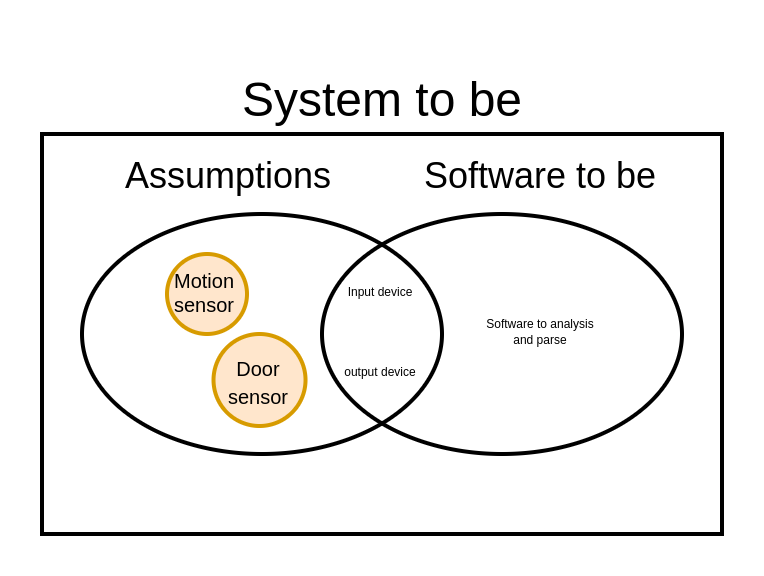
\includegraphics[width=0.5\textwidth]{images/system_to_be.png}
    \caption{مهندسی نیازمندی بیشتر به \lr{Assumption} و قسمت اشتراکی شامل می‌شود.}
    \label{fig: systemToBe}
\end{figure}

\subsubsection{مفهوم \lr{Definition}}

یک معنای دقیق از چیزایی است که می‌نویسم به عبارت دیگر تمام اصطلاحاتی که در سیستم
می‌تواند وجود داشته باشد را بیان می‌کند.

\subsubsection{مفهوم مانیتور کردن}

مانیتور کردن یعنی بررسی داده‌های ورود و انجام تحلیل روی آنها.

\subsubsection{مفهوم کنترل کردن}

کنترل کردن یعنی فرایند بعد از تحلیل، یعنی اعمال کردن نتایج بدست آمده.

\subsubsection{عوامل \lr{Descriptive}}

عوامل توصیفی، قوانین طبیعی و قید و شرط‌های فیزیک که غیر 

\subsubsection{ویژگی دامنه یا \lr{Domain property}}

یک عبارت توصیفی است که یک حقیقت از فیزیک را بیان می‌کند. این عبارت قابل مذاکره
نیست که برای مثال بگوییم بعداً می‌توان آن را تغییر داد. به هیچ وجه نمی‌توان آن
را کم یا زیاد کرد.

برای مثال:

\begin{enumerate}
    \item برای مثال دانشجو نمی‌تواند دو درس مختلف در زمان یکسان اخذ کند. یعنی از
    نظر فیزیک نمی‌توان همزمان در دو کلاس در زمان یکسان حاضر شد. و این پیام را
    نیازمندی نرم‌افزار در حقیقت برنامه نویس مشخص می‌کند.
    \item هنگامی که در‌های قطار بسته باشند، یعنی دیگر باز نیستند.
    \item اگر شتاب قطار مثبت باشد، بدان معانست که سرعت قطار =! صفر می‌باشد.
\end{enumerate}

\subsubsection{دامنه‌ها}

دامنه‌های در دل سازمان‌ها هستند، مانند دامنه پژوهشی، دامنه‌های مالی و ارتباط بین
آدم‌ها در دامنه وجود دارد.

\subsubsection{اسکوپ‌ها}

مجموعه‌هایی از \lr{System requirement} هستند که نرم‌افزار می‌تواند در آنها ورود
داشته باشد. مثلا فعالیت‌های مربوط به ثبت‌نام دانشجو، که اصطلاحاً به آنها
\lr{System scope} می‌گویند. به عبارتی دیگر، مجموعه‌ای از قابلیت‌ها که در
\lr{Domain property} تعریف می‌شود.

\subsubsection*{نکات}

\begin{itemize}
    \item مهندس نیازمندی باید در کنترل و مدیریت اسکوپ‌ها حساسیت داشته باشد که
    نرم‌افزار از دست خارج نشود و باعث پیچیده‌تر شدنش نگردد.
    \item دامنه‌ها درست است که ثابت و غیرقابل مذاکره هستند، اما از یک دامنه به
    دامنه دیگر می‌تواند ویژگی‌ها تغییر کنند در حالی که ساختار این دامنه حفظ شود.
    برای مثال زمانی که دامنه مورد نظر یک کتابخانه فیزیکی است، همزمان دو نفر
    نمی‌توانند یک کتاب مشترک را تقاضا کنند. اما در کتابخانه دیجیتال که به صورت
    اپلیکیشن می‌باشد، درست است که ساختار دامنه همانند موجودیت‌ها و شکل کتابخانه
    فیزیکی است اما نحوه استفاده آن کاملاً تغییر کرده و چندین کاربر می‌توانند
    همزمان یک کتاب را به صورت دیجیتال مطالعه کنند.
    \item در مهندسی نیازمندی تنها یک نمودار استفاده نمی‌شود. برای مثال زمانی که
    یک نمودار \lr{Sequence} برای نمایش ارتباطات دستگاه ها کشیده می‌شود نیازمند
    آن است که نمودار هدف نیز داشته باشد. بعد از آن بایستی تمام ریسک‌های مربوط به
    آن نیز به صورت نمودار اعلام شود. چرا که باعث تولید یک سند مهندسی نیازمندی
    کامل می‌شود که در زمان‌های مختلف می‌توان به آن مراجعه کرد و متوجه تمام
    موضوعات بدون فراموشی تنها یک بخش شد.
    \item بُعد \lr{Why} در نمودار معمولاً نشان‌دهنده اهداف است. مثلا پیاده‌سازی این
    قابلیت هدف‌اش رضایت مشتری است.
    \item همیشه از اهداف شروع می‌کنیم و به نیازمندی‌های سیستمی می‌رسیم و
    نیازمندی سیستمی را در نیازمندی‌های نرم‌افزاری و محیطی بررسی می‌کنیم.
\end{itemize}

\begin{figure}[H]
    \centering
    \begin{forest}
        [Goal
            [
                [System requirement
                    [
                        Software requirement
                    ]
                    [
                        Assumption
                    ] 
                ] 
                [System requirement
                    [
                        Software requirement
                    ]
                    [
                        Assumption
                    ] 
                ] 
            ]
        ]
    \end{forest}
\end{figure}

\subsubsection{تفاوت‌های بین \lr{Descriptive} و \lr{Prescriptive}}

\begin{itemize}
    \item جملات تجویزی را می‌توان برای آنها مذاکره کرد، آنها را کم و زیاد کرد یا
    حتی برای آنها جایگزینی معرفی نمود.
    \item جملات توصیفی اصلاً قابل تغییر نیستند.
\end{itemize}

\subsection{مولفه‌های مربوط به نیازمندی نرم‌افزار در نیازمندی سیستم}

\begin{enumerate}
    \item مانیتورینگ: تمام مقادیر محیطی که نرم‌افزار توسط دستگاه‌های ورودی مانند
    سنسور‌ها، داده‌های آن را دریافت می‌کند.
    \item کنترل: مقادیر محیطی که نرم‌افزار آنهارا می‌تواند از طریق دستگاه‌های
    خروجی (Actuators) آن‌ها را کنترل (اعمال) کند.
    \item مقادیر دستگاه‌های ورودی \footnote{Input}: تمام داده‌هایی که به عنوان
    ورودی در نرم‌افزار استفاده می‌شود.
    \item متغیر‌های خروجی \footnote{Output}: مقادیری که نرم‌افزار آنها را در
    دستگاه‌ّای خروجی اعمال می‌کند.
\end{enumerate}

\subsubsection*{نکته}

بیشتر سازمان‌ها به دو دسته زیر فعالیت‌های خودشان را انجام می‌دهند:

\begin{enumerate}
    \item سازمان‌هایی که هدفگرا هستند و تنها برای رسیدن به محصول آخرین تلاش و
    فعالیت خود را می‌کنند.
    \item سازمان‌هایی که تعداد \lr{Agent} و کاربرانشان زیاد است و ارزش‌های زیادی
    برای آنها قائل می‌شوند به صورت Agentگرا یا عاملگرا هستند.
\end{enumerate}

سطح \lr{System requirement} بالا می‌باشد، چرا که مشتری تنها درخواست می‌کند که
می‌خواهد چنین قابلیت‌هایی وجود داشته باشد، به ماهیت و نیازمندی و حتی پیچیدگی
آنها کاری ندارد.

\subsection{توافق بر لغات}

\begin{enumerate}
    \item \lr{SOFTREQ}: منظور \lr{Software requirement}
    \item \lr{ASM}: منظور مفروضات یا \lr{Assumption}
    \item \lr{DOM}: منظور دامنه یا \lr{Domain}
\end{enumerate}

\begin{equation}
    SOFTREQ + ASM + DOM \rightarrow SYSTEMREQ
\end{equation}

اگر نیازمندی نرم‌افزار، مفروضات و دامنه‌ها همگی مقید و راضی باشند نیازمندی سیستم
نیز بدست می‌آید. با استفاده از پارامتر‌های بالا می‌توان به سیستم نهایی رسید.

\begin{figure}[H]
    \centering
    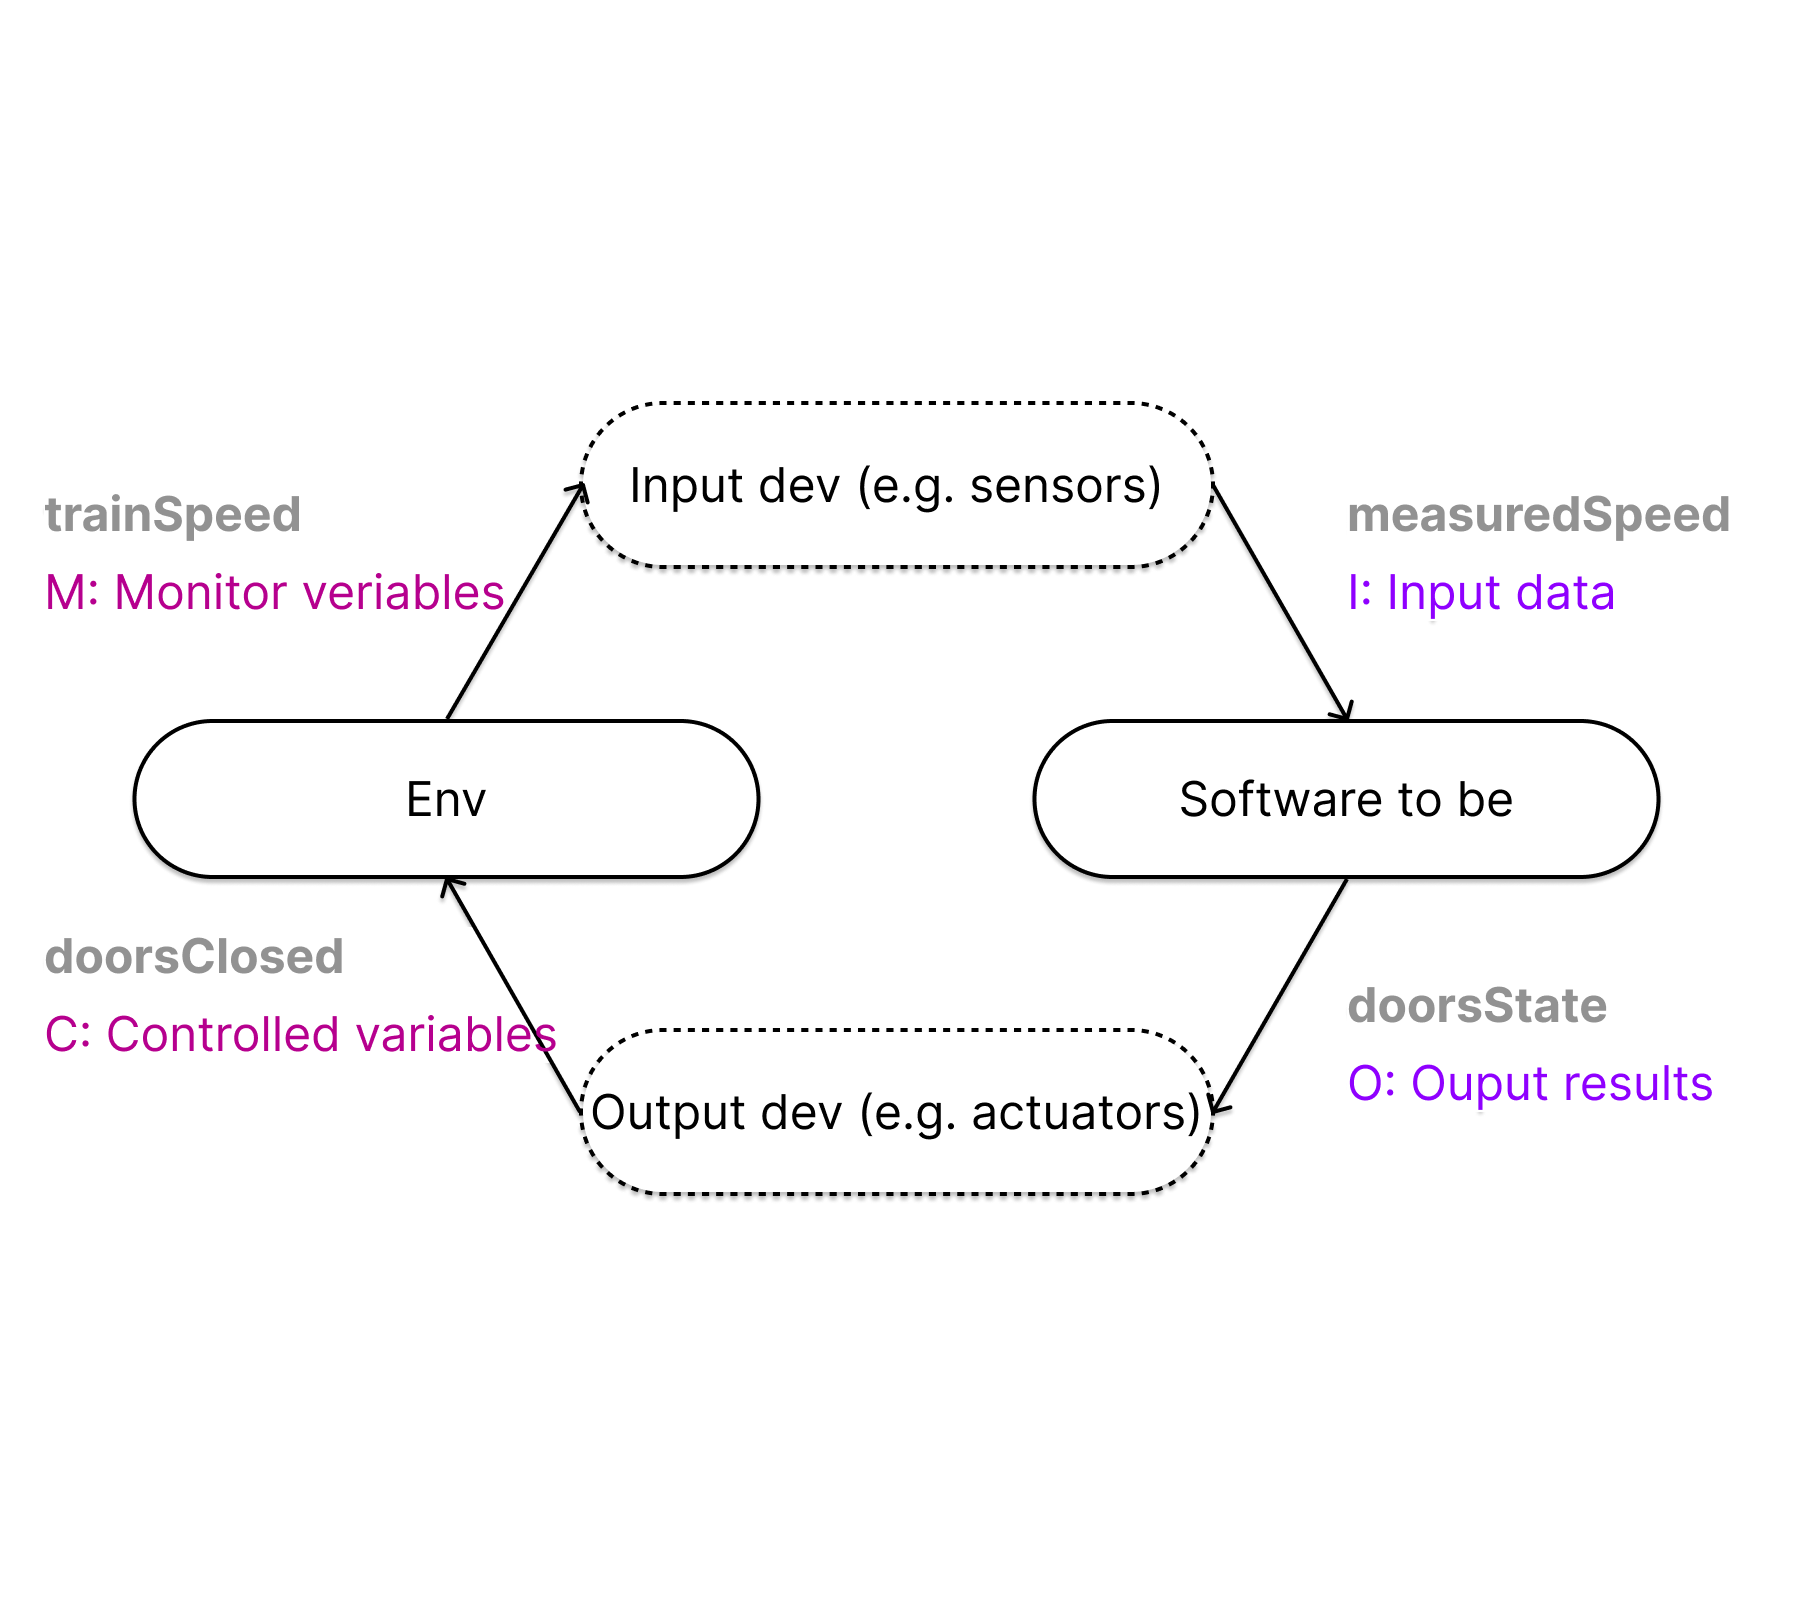
\includegraphics[width=0.7\textwidth]{images/train_sysreq.png}
    \caption{ارتباط نیازمندی سیستم در نرم‌افزار به همراه استدلال‌ها}
    \label{fig: }
\end{figure}


\begin{LTR}
    \begin{itemize}
        \item \lr{SOFTREQ}: Input ` Ouput
        \item \lr{ASM1}: Monitor ` Input
        \item \lr{ASM2}: Ouput ` Control
        \item \lr{SYSREQ}: Monitor ` Control
    \end{itemize}
\end{LTR}

\subsection*{استدلال سناریو}

\begin{equation}
    SOFTREQ: measuredSpeed \neq 0 \rightarrow doorsState = "closed"
\end{equation}

\begin{equation}
    ASM1: measuredSpeed \neq 0 iff trainSpeed \neq 0
\end{equation}

\begin{equation}
    ASM2: doorsState = "closed" iff doorsClosed
\end{equation}

\begin{equation}
    DOM: trainMoving iff trainSpeed \neq 0 
\end{equation}

\begin{equation}
    SYSREQ: trainMoving \rightarrow doorsClosed 
\end{equation}

\subsection{دسته‌بندی نیازمندی‌ها}

\subsubsection{\lr{Functional requirement}}

تعیین می‌کند که چه سرویسی قرار است در \lr{Software to be} ارائه شود. برای مثال:

\begin{itemize}
    \item نرم‌افزار کنترل قطار باید بتواند سرعت تمام بخش‌های سیستم قطار را کنترل
    کند.
    \item سیستم آنلاین فهرست کتب باید براساس موضوع کتاب نام تمام کتابخانه را
    نمایش دهد. 
    \item کاربران در سیستم پارکینگ آنلاین باید بتوانند رزرو لحظه و رزرو روزانه
    را به انتخاب خودشان استفاده کنند.
    \item دانشجویان زمانی که وارد کلاس آنلاین می‌شوند باید قابلیت به اشتراک
    گذاری صفحه نمایش خود را داشته باشند.
\end{itemize}

همچنین می‌توانند براساس شرایط محیطی باشند که تحت آن چه عملیاتی باید انجام شود:

\begin{itemize}
    \item در‌های قطار تنها در زمانی می‌توانند باز شوند که قطار به طور کامل ایستاده باشد.
\end{itemize}

\subsubsection*{دسته‌بندی توابع}

\begin{enumerate}
    \item \lr{Information}: اطلاع رسانی، اعلانات هر چیزی که قابلیت ارسال و
    دریافت را داشته باشد.
    \item \lr{Satisfaction}: تعیین \lr{State} یک کار است که در جریان معنا دارد.
    \item \lr{Stim-response}: محرک پاسخ، وقتی دکمه در \lr{UI} زده شد آلارم را
    صدا کند.
\end{enumerate}

\subsubsection{\lr{Non-functional requirement}}

تعیین می‌کنند که چگونه یک سرویس می‌تواند ارائه شود. برای این دسته باید مجموعه‌ای
از اقدامات که بار اجرایی دارند را استفاده کرد:

\begin{itemize}
    \item معیار‌ها و نیازمندی‌های کیفی:
    \begin{itemize}
        \item معیار‌های ایمنی
        \item معیار‌‌های امنیتی
        \item سرعت و دقت
        \item عملکرد زمانی و حافظه‌ای
        \item قابلیت استفاده
    \end{itemize}
    \item بقیه موارد
    \begin{itemize}
        \item هنجار‌ها
        \item معماری
        \item نیازمندی‌های توسعه 
    \end{itemize}
\end{itemize}

برای مثال:

\begin{itemize}
    \item دانشجویان هنگام به اشتراک گذاری صفحه خود کیفیت صوت را به خوبی قبل از
    اشتراک گذاری داشته باشند.
    \item قطار هنگام حرکت امکان باز کردن در را نداشته باشد.
    \item دستورات شتاب قطار هر ۳ ثانیه یکبار می‌تواند ارسال شود.
\end{itemize}

\subsection{کیفیت سرویس‌دهی یا \lr{QoS} (محصول)}

پارامتری را نشان می‌دهد که می‌خواهیم آن را از نظر کیفی تامین کنیم. برای مثال
برقراری اهداف امنیتی.

\subsection{\lr{Service Level Agreement}}

یک توافق بین معمار نرم‌افزار و کارفرما برای تعیین سطح سرویس از نظر کیفی می‌باشد.
در قرار‌داد‌های \lr{SLA} مقدار قابل قبولی از \lr{QoS}هایی که دنبالش هستیم را
بیان می‌کنیم.

\subsection{تفاوت بین \lr{Constraint} و \lr{Limitation}}

\lr{Constraint} به معنای قید و شرط است، مقید شدن به چیزی. برای مثال نرم‌افزاری
توسعه داده شود که قابلیت نصب روی دستگاه‌های موبایل را داشته باشد.

\lr{Limitation} به معنای محدودیت است که بار منفی دارد. در این حالت نرم‌افزار
باید با آن کنار بیاید.

\subsection{مفهوم هنجار‌ها یا \lr{Compliance} (محصول)}

منظور از \lr{Compliance} قواعد و هنجار‌هایی است که الزاما ثابت نیستند. نرم‌افزار
باید تابع این هنجار‌ها باشد. قواعدی که در نرم‌افزار قید می‌شود برای مثال فاصله
بین دو ماشین در سال ۲۰۲۰ با تصمیم‌گیری شهرداری برای ماشین‌های خودران ۴ متر توافق
شد. اما بعد از پیشرفت تکنولوزی و علوم مربوطه این فاصله به یک متر کاهش یافت.

\subsection{قید‌های معماری \lr{Architectural constraint} (محصول)}

بعضی از قید‌های معماری مربوط به نصب و راه‌اندازی هستند و برخی دیگر مربوط به
توزیع می‌باشند.

\begin{enumerate}
    \item نصب
    \begin{enumerate}
        \item نرم‌افزار باید روی پلتفرم موبایل یا عینک گوگل قابل نصب باشد
        \item مشخصات لازم برای نصب موفقیت‌آمیز نرم‌افزار و بازی
        \item این نیاز می‌تواند پایین‌تر از سطح سکو نیز باشد، مثلاً نصب تنها در
        یک سیستم عامل مخصوص
        \item قابلیت نصب تنها در سخت‌افزار‌های X86
    \end{enumerate}
    \item قید توزیع: ورودی و خروجی از دو درب مختلف در دانشگاه، به دلیل آنکه
    داده‌های محیطی ورودی و خروجی در دو محل متفاوت است برای رسیدن به توافق در این
    توزیع باید این داده‌ها را در یک جا با هم سینک کنیم تا اطلاعات ورودی و خروجی
    مناسب یکدگیر پدید آید.
\end{enumerate}

\subsection{قید‌های توسعه \lr{Development constraint} (مدیر پروژه)}

یکی از مهم‌ترین عوامل نگرانی مدیر پروژه است، کاری به ماهیت محصول ندارد بلکه برای
او مهم‌ترین عوامل انتخاب مناسب متدولوژی و تصمیم درست می‌باشد. تعیین هزینه زمانی
و مالی نیز از دیگر نگرانی‌های مدیر پروژه می‌باشد تا در نهایت طراح معماری بتواند
با دید کامل و بدون تحت فشار قرار گرفتن، معماری مناسب را طراحی کند.

\subsection{فرایند و مراحل مهندسی نیازمندی‌}

برای ساخت سبد دامنه خود نیازمند انجام فرایند مهندسی نیازمندی هستیم. این فرایند
چهار قدم اصلی را بیان می‌کند. مهم‌ترین ویژگی این فرایند مراحل آن هستند که
می‌توانند به صورت تکرار پذیر انجام شوند. حرکت در بین این فرایند به صورت ساعتگرد
می‌باشد.

\begin{figure}[H]
    \centering
    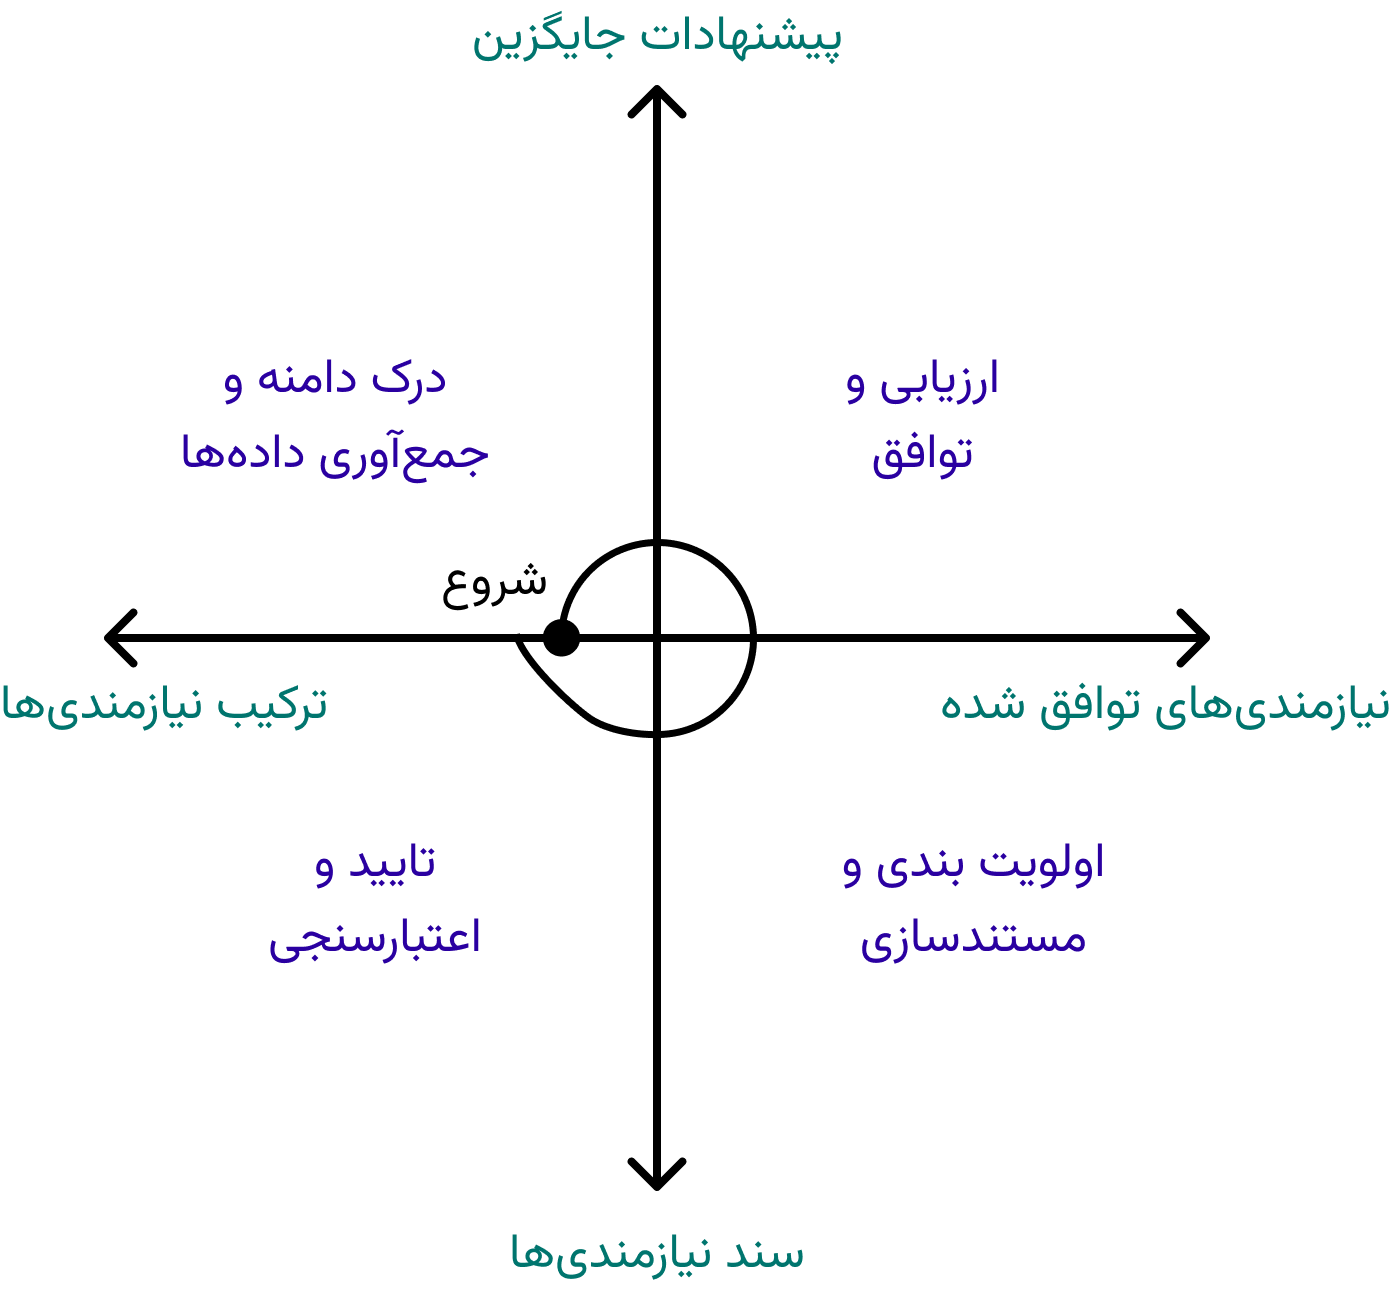
\includegraphics[width=0.5\textwidth]{images/re_process.png}
    \caption{مراحل مهندسی نیازمندی‌ها}
    \label{fig: reProcess}
\end{figure}

\subsubsection{پیشنهادات جایگزین، درک دامنه و جمع‌آوری داده‌ها}

این بخش با دامنه‌ها و استخراج نیازمندی‌ها ارتباط دارد. یعنی مهم‌ترین وظیفه در
این ناحیه جمع‌آوری داده‌ها می‌باشد. سعی می‌کنیم تمام سناریو‌ها را بررسی کنیم و
به لیستی از داده‌های در رابطه با دامنه خواسته‌های مشتری برسیم. به یاد داشته
باشیم که داده‌های جمع‌آوری شده صرفا همه آنها مفید نمی‌باشد پس نتیجه می‌گیریم که
این لیست قابل تغییر و حذف می‌باشد که به داده‌های اصلی برسیم. برای مثال وقتی در
حال جمع‌آوری داده برای توسعه سیستم مالی هستیم با داده‌های بخش بایگانی هم رو به
رو خواهیم شد که هیچ ارتباط مستقیمی با سناریو‌های مالی ندارد پس می‌توانیم از
جمع‌آوری داده در بخش بایگانی صرف نظر کنیم.

\subsubsection{نیازمند‌های توافق شده، ارزیابی و توافق}

همانطور که از نامش پیداست در این ناحیه به تجزیه و تحلیل و ارزیابی داده‌ها
می‌پردازیم. به گونه‌ای که سعی می‌کنیم داده‌هایی که نامربوط به \lr{Scope} می‌باشد
را شناسایی کنیم و آنها را حذف کنیم. هر خواسته‌ای در \lr{Scope} مشتری می‌تواند
ریسک‌هایی باشد که به عنوان قابلیت در نرم‌افزار می‌خواهد پیاده شود.

\begin{itemize}
    \item قضیه برنامه \lr{LMS} را در نظر داشته باشید. کلاس آنلاین به حضور
    دانشجویان نیاز دارد و قابلیت‌هایی در خصوص عضویت آنها در این سامانه وجود دارد
    اما ریسکی که در این میان به وجود می‌آید آن است که ممکن است اینترنت قطع شود و
    دسترسی دانشجویان به این سامانه با مشکل مواجه شود.
\end{itemize}

سوالی که در این میان مطرح می‌شود آن است که آیا تمام نیازمندی‌هایی که به سیستم
وارد می‌شود الزاماً هم‌راستا می‌باشد؟

پاسخ به این سوال خیر می‌باشد چرا که ممکن است نیاز دو \lr{Assumption} با یکدیگر
تداخل داشته باشد.

\begin{itemize}
    \item قضیه کارنامه را به یاد داشته باشید. درخواست مشتری اول (استاد) آن است
    که فقط او بتواند در هنگام ثبت نمره کارنامه را دسترسی داشته باشد. در راستای
    آن مشتری دوم (دانشجو) هم دقیقاً همین نیاز را دارد. این دو نیاز هم‌راستا
    نمی‌باشد چرا که اگر یکی را تنها برای یک نوع مشتری برآورده کنیم ممکن است با
    مشتری دیگر تداخل یا \lr{Conflict} ایجاد شود.
\end{itemize}

\subsubsection{سند نیازمندی‌ها، اولویت‌بندی و مستندات}

وقتی به این مرحله رسیده‌ایم یعنی با دو مرحله قبلی در نیازمند‌های مشتری به اجماع
رسیده‌ایم. یک سبدی از \lr{Scope}ها که خیلی آشفته بود به یک سبدی تبدیل می‌شود که
همه افراد روی آن توافق دارند. این توافق‌ها در سند نیازمندی نوشته می‌شوند. این
سند یک قالب استاندارد دارد و در این قالب مشخص می‌شود که با چه ابزاری باید کار
کنیم، چگونه بنویسیم و نماد بصریمان به چه شکلی باشد. بعد از این توافق‌ها این سند
به طراح معماری نرم‌افزار تحویل داده می‌شود. این سند با نمودار‌های بصری‌اش زبان
مشترک بین طراح و مهندس نیازمندی است تا مطالب صریح و سریع به طراح معماری منتقل
شود.

\subsubsection{نیازمندی‌های ترکیبی،‌ تایید و اعتبارسنجی}

سبدی که تا الان آماده شده است می‌تواند دستخوش تغییرات باشد تا به حدی که به ۸۰
درصد نیازمندی‌های ثابت و ۲۰ درصد نیازمندی‌هایی که باید تغییر کنند یا بروز شوند.
این تغییر ۲۰ درصدی می‌تواند بخش‌های صحیح را هم تحت تاثیر خودش قرار دهد (اشاره به
قضیه \lr{Side effect}). پس در هر بار ایجاد تغییر در نیازمندی‌ها بایستی در ابتدا
اعتبارسنجی شوند و تایید ایجاد تغییرات را دریافت کند.

\subsubsection*{نکته}

مراحل نیازمندی‌ها می‌تواند چندین دور حلقوی داشته باشد تا همه موارد دخیل در آن به
نسخه پایدار خود برسند.

\subsection{نیازمندی‌ها در چرخه توسعه نرم‌افزار}

سوال: آیا هر سیستمی نیازمند مهندسی نیازمندی می‌باشد؟

خیر، سند نیازمندی برای سازمان‌ها با سیستم بزرگ (سیستم‌های \lr{Legacy}) کاملاً
مورد احتیاج می‌باشد. به طور کل سازمان‌هایی که جریان کاری (\lr{Workflow}) اصلی را
اداره می‌کنند نیازمند سند نیازمندی هستند. پروژه‌های استارتاپی که به مردم خدمت
می‌کنند در اصل جنس خدمت با دیگر سازمان‌ها یکی است اما نحوه انجام آن متفاوت
می‌باشد. این سیستم‌ها هم سند نیازمندی برایشان اهمیت دارد.

به خاطر داشته باشید که سند نیازمندی قابلیت استفاده مجدد را به پروژه‌های مشابه
می‌دهد. به طور کلی گفتنی است که سند نیازمندی یک منبعی برای پروژه‌های مشابه
می‌باشد نه یک الگو.

به طور کلی، در سند نیازمندی، خواسته‌های مشتری تحلیل و جمع‌آوری می‌شود و بعد
قرارداد در پروژه پیاده‌سازی می‌شوند.

\subsection{\lr{Request for Proposal} یا \lr{RFP}}

سازمان‌ها بر اساس \lr{RFP} کار می‌کنند. مهندس نیازمندی و متخصصین با هم روی این
سند بر اساس خواسته‌های مشتری توافق می‌کنند که کار خودشان را شروع کنند. معمولاً
واحد‌های \lr{IT} مسئول این اسناد هستند.

\subsection{تعریف: به اجماع رسیدن مطالب از سند نیازمندی}

سند نیازمندی یا \lr{Requirement Document} محصول اصلی فرایند مهندسی نیازمندی است.
در آن سیستمی که می‌خوایم در آینده داشته باشیم (\lr{System-to-be}) به شکل اهداف
\footnote{\lr{Objectives}}، قید و بند‌ها \footnote{\lr{Constraints}}، مفاهیم
ارجاع داده شده، تسک‌ها و تکالیف مشخص شده، نیازمندی‌ها، فرضیات
\footnote{\lr{Assumption}} و ویژگی دامنه‌های مربوطه تعریف شده است.

\subsection{تاثیراتی که سند نیازمندی به فرآورده‌های نرم‌افزاری دارد}

\begin{itemize}
    \item \lr{Prototype}:
    \item \lr{Project estimations (Size, Cost, Shedules)}: یکی از نیازمندی‌های
    غیرعملیاتی مربوط به توسعه است که روی سبد \lr{Scope}ها تاثیر گذار می‌باشد. در
    این قسمت رابطه سند نیازمندی با آن دو طرفه می‌باشد تا مشخص کنیم برای
    نیازمندی‌های خود چقدر زمان، چه مقدار هزینه و چه تعداد نیروی انسانی به طور
    مثال تعیین کنیم. در این قسمت سند نیازمندی ممکن است چند بار دستخوش تغییرات
    قرار گیرد و اصطلاحاً نسخه‌بندی شود. ممکن است در نسخه اولیه نیاز ما با زمان
    مطابقت داشته باشد اما به علت بزرگ شدن پروژه و بروز شدن خواسته‌های مشتری،
    دیگر این زمان با نیازمندی‌های جدید سازگاری ندارد و بایستی بروز شود.
    \item \lr{Architectural design}:
    \item \lr{Software quality assurance}:
    \item \lr{Implementation and integration}:
    \item \lr{Documentation}: 
    \item \lr{Maintenance}:
\end{itemize}

% پروتوتایپ در خصوص بخری نیازمندی‌ها که مبهم است که واضح نیست یک پروتوتایپ درست
% می‌کنیم که بفهمیم اون نیاز چیست. می‌تواند روی کاغذ باشد باشد یا یه ui اشد. که
% منظور اولیه رو برساند. می‌تواند تو سطح فاکنشن باشد هم می‌تواند نان فانکشن باشد.

% چرا این سند دو طرفه‌است. توی محیط یه چیزی به ما گفتن. یعنی یه نیازی به ما منقل
% شده که ما پروتوتایپ درست کردیم. بعد اون پروتوتایپ رو بهش نشون میدیم که ببینیم
% درست فهمیدیم یا نه. ممکن نیازمندی اضافه بشه یا حذف بشه تا سبد اسکوپ ما کامل شود.

% acceptance test باید با نیازمندی‌های مشتری مطابقت داشته باشد. باید سناریو تست
% وجود داشته باشد. سناریو‌های تست از سند نیازمندی می‌آید.

% معماری:

% چه قید‌هایی، چه ترتیبی تا بتواند نان فانکشن‌ها رو چک کنه که نان فانکشن‌ها در سند
% نیازمندی نوشته شده است. مانند availability, useability, و دیگر خواسته‌ها.

% معماری یکسری الزامات را ایجاد می‌کند. اون الزامات از جنس فانکشن‌هاستند. که روی
% سند نیازمندی‌ها تاثیر می‌ذاره.

% ریپورت صفحه ۵۳ نمودار رو نگاه اینجا بنویس.

% expectation منظور همان Assumptionهاست.

\section{فصل دوم، درک دامنه و جمع‌آوری نیازمندی‌ها}

این فصل معادل فاز (فرایند) اول مهندسی نیازمندی یعنی استخراج داده‌ها می‌باشد.
تمام مشکلاتی که در \lr{Scope} می‌باشد در حقیقت \lr{System as is} را مشخص می‌کند.

\subsection{دسته‌بندی جمع‌آوری داده}

جمع‌آوری داده‌ها را می‌توانیم به دو دسته زیر تقسیم کنیم، (درک دامنه و جمع‌آوری
داده‌ها ترکیبی از تکنیک‌های متفاوت می‌باشد):

\begin{enumerate}
    \item تکنیک‌های فرآورده‌گرا یا \lr{Artifact driven}: هر آن چیزی که در پروژه
    تولید یا استفاده می‌شود.
    \item \begin{enumerate}
        \item می‌توانیم از قواعد آموزشی نیازمندی‌هایی را خارج کنیم.
        \item \lr{Prototype}ها
        \item مستندات موجود در سازمان‌ها
    \end{enumerate}
    \item تکنیک‌های ذینفع‌گرا یا \lr{Stakeholder driven}: هر آن چیزی که در
    ارتباط با آدم‌ها در سازمان باشد.
    \item \begin{enumerate}
        \item جلسات
    \end{enumerate}
\end{enumerate}

\subsection{تکنیک‌های جمع‌آوری اطلاعات فرآورده‌گرا}

\subsubsection{\lr{Background study}}

\begin{itemize}
    \item سازمان: نمودار‌های سازمانی، بیزینس پلن‌ها، گزارش‌های مالی، صورتجلسه
    \footnote{\lr{Meeting minutes}}
    \item دامنه‌ها: کتاب‌ها، نظرسنجی‌ها، مقالات، مقررات و استاندارد‌ها،
    گزارش‌های سیستم‌های مشابه در دامنه مشابه
    \item سیستم کنونی یا \lr{System as is}: جریانات کاری مستند شده، فرایند‌ها،
    قوانین بیزینسی، مستندات مبادله شده، گزارش‌های مربوط به شکایات، مستندات مربوط
    به تغییر خواسته‌های مشتری و غیره.
\end{itemize}

یکی از نیازمندی‌های مهم برای ذینفعان می‌باشد تا آن‌ها را نسبت به جلسه بعدی‌شان
آماده کند.

مهم‌ترین مشکلات:

\begin{enumerate}
    \item حجم مستندات به شدت زیاد است
    \item جزئیات نامرتبط برای مثال بخش بایگانی اسنادی را نگهداری می‌کند که ممکن
    است کاملاً با یکدیگر نامرتبط باشد.
    \item اسناد ممکن است منسوخ شده یا \lr{Outdated} باشند.
\end{enumerate}

راه حل مشکلات این بخش:

استفاده از تکنیک هرس کردن مستندات می‌باشد. بررسی بخش‌هایی که معتبر است و حذف
بخش‌هایی که منسوخ شده و غیرمعتبر می‌باشد. این تکنیک مانند خواندن فصل‌های مشخص
شده از یک درس می‌باشد تا اینکه کل فصل‌های مطرح شده را بخواند.

\subsubsection{\lr{Data collection, questionnaires}}

جمع‌آوری داده‌هایی که مستندسازی نشده‌اند. مانند حقایق و ارقام. حقایق و ارقام به
صورت صریح در مستندات موجود نیستند. این داده‌ها می‌تواند به صورت \lr{Meta data}
با شد مانند فرم ثبت‌نام، جمله ندارد بلکه براساس داده‌ها می‌توان به یک جمله رسید.
بر اساس داده‌هایی که جمع‌آوری کرده‌ایم می‌توانیم جملات \lr{Functional} بنویسم.
نوشتن جمله و تفسیر توسط مهندس نیازمندی‌ها بر اساس داده‌های جمع‌آوری شده انجام
می‌پذیرد.

این داده‌ها مانند موارد زیر می‌باشد:

\begin{itemize}
    \item داده‌های مربوط به دیجیتال مارکتینگ، آمار استفاده، ارقام اجرایی و
    عملکردی، هزینه‌ها
    \item استفاده از تکنیک‌های نمونه‌گیری آماری
\end{itemize}

\subsubsection*{مشکلات}

\begin{itemize}
    \item ممکن است تفسیر مهندس نیازمندی لزوماً درست نباشد.
    \item داده کاوی مطمئن و درست ممکن است بسیار زمانبر باشد.
\end{itemize}

در روش قبل که اسنادی که می‌خواندیم اسناد عملیاتی بودند اما در این روش اسنادی که
مطالعه می‌شود کاملاً غیرعملیاتی هستند (مانند معیار‌ها و کیفیت ارائه سرویس).

\subsubsection*{روش‌های احتمالی}

\begin{itemize}
    \item \lr{requirement elicitation}
    \item \lr{Text mining}
\end{itemize}

\subsubsection*{پرسشنامه}

لیستی از سوالاتی که توسط ذینفعان مشخص شده را آماده می‌کنیم که هر کدام یک جواب
مناسب را می‌تواند در برگیرد.

نمونه‌ها میتواند:

\begin{itemize}
    \item انتخاب یک گزینه از چند گزینه. مانند استفاده از \lr{Radio button}
    \item سوالاتی که وزن‌دار هستند:
    \item \begin{itemize}
        \item کیفی: عالی، خوب، بد
        \item کمی: اعلام مقدار به صورت درصدی
    \end{itemize}
\end{itemize}

\subsubsection*{ویژگی‌های یک پرسشنامه خوب}

\begin{enumerate}
    \item تنوع زیاد کاربران و عدم تمرکز موقعیت مکانی و فرهنگ مختلف که در تمام
    کاربران متغیر می‌باشد. پس برای پوشش تنوع و گوناگونی
    \footnote{\lr{Diversity}} کاربران از پرسشنامه استفاده می‌کنیم.
    \item سریع، ارزان و قابل دسترس از راه دور نیازمندی بسیاری از کاربران را
    جمع‌آوری می‌کنیم.
    \item پرسشنامه‌ای خوب است که روایی و کارایی داشته باشد.
\end{enumerate}

\subsubsection*{تفاوت پایایی و روایی در پرسشنامه‌ها}

یک پرسشنامه خوب باید دو ویژگی پایایی و روایی را به همراه داشته باشد. 

\begin{itemize}
    \item پایایی قابلیت اطمینان پرسشنامه به همراه دقت در اندازه‌گیری می‌باشد.
    یعنی اگر همان پرسشنامه در همان شرایط بخواهد به صورت مجدد صورت گیرد، امتیاز
    یا مقدار حاصل از پرسشنامه هیچ تغییری نخواهد کرد.
    \item روایی به معنای آن است که میزان مطابقت نتایج بدست آمده از پرسشنامه با
    دنیای واقعی به چه اندازه‌ای می‌باشد.
\end{itemize}

\subsubsection{\lr{Repertory grids, Card sorts for concept acquisition}}

جمله مجموعه‌ای از اسم‌ها را با فعل به یکدیگر متصل می‌کند تا یک جمله کامل را
تشکیل دهد. برای مثال جمله «دانشجو باید بتواند درس انتخاب کند.» اسم‌ها به ترتیب،
«دانشجو» و «درس» هستند و فعل این جمله که این دو اسم را به یکدیگر متصل می‌کند
«انتخاب کردن» می‌باشد.

اسم‌ها تبدیل به کارت می‌شوند و تمام کارت‌ها معادل به کلاس هستند. تمام کلاس‌ها در
فضای مسئله بررسی می‌شوند و فضای راه‌حل در حقیقت خروجی ارتباط آنها (جمله) است.
یکی از مثال‌های فضای راه‌حل اتصال به دیتابیس می‌باشد.

\subsubsection*{فضای مسئله}

دقیقاً وضعیت موجود را نمایش می‌دهد. تمام چیز‌هایی که می‌بینیم در حقیقت فضای
مسئله می‌باشد.

\subsubsection*{فضای راه‌حل}

فضای راه‌حل نتیجه ارتباط جملات و کلاس‌ها هستند که طراح مشخص می‌کند.

\subsubsection*{مثال}

برای مثال می‌توان به دانشجو و شماره دانشجویی اشاره کرد. نام و نام خانوادگی،
تاریخ تولد، سال ورودی دانشگاه، رشته ورودی، گرایش رشته و غیره تمام مسائلی هستند
که موجودیت دانشجو را تعریف می‌کنند پس فضای مسئله می‌باشند.

طراح سیستم دانشگاهی با توجه به این فضای‌ مسئله ورودی‌ها را بررسی می‌کند و یک
خروجی برای مشخص کردن یکتا بودن دانشجو تولید می‌کند و آن هم شماره دانشجویی
می‌باشد که یکی از مهم‌ترین فرآورده‌های فضای راه‌حل است.

\subsubsection*{نکته}

کاملاً بستگی به نیاز سیستم دارد که مشخص کنیم یک اسم کلاس باشد یا نه. زیرا یک اسم
هم می‌تواند کلاس باشد یا می‌تواند به عنوان ویژگی کلاس دیگری یا \lr{Attribute}
باشد. برای مثال کتابخانه می‌توان اشاره کرد که اگر بخواهیم «کتاب‌ها» و
«نویسندگان» را کلاس جداگانه در نظر بگیریم می‌توانیم کوئری‌هایی در این بابت داشته
باشیم که یک کتاب را چه نویسندگانی تالیف کرده‌اند و یا یک نویسنده چه کتاب‌هایی
دارد. یا می‌توانیم نیاز سیستم را در این ببینیم که یکی از \lr{Attribute}های کتاب
نویسنده باشد به جای آن که یک کلاس جداگانه داشته باشد.

در حالت کلی می‌توان گفت که قانون سفت و سختی برای تشکیل کلاس از روی کارت‌ها وجود
ندارد و کاملاً نیاز سیستم مشخص می‌کند که کلاس باشند یا \lr{Attribute}.

\subsubsection*{گریدبندی کردن کارت‌‌ها}



% \subsubsection{\lr{Scenarios, Storyboards for problem world exploration}}

% \subsubsection{\lr{Prototypes, Mock-ups for early feedback}}

% \subsubsection{\lr{Knowledge reuse: Domain-independent, Domain specific}}

% \subsection{تکنیک‌های جمع‌آوری اطلاعات ذینفع‌گرا}

% \subsubsection{\lr{Interviews}}

% تمام سوالاتی که برای آن‌ها جوابی نداریم را در بخش \lr{Interview} می‌پرسیم. مثلا
% بعد از ثبت‌نام کاربر برای او اعلاناتی ارسال شود؟ یا مثلاً می‌گویم که در سناریو
% تغییر کلاس کاربر اعلانات ارسال شود.

% \subsubsection{\lr{Observation and ethnographic studies}}

% \subsubsection{\lr{Group sessions}}
\newpage

\section{فصل سوم}

در فصل یک و دو در مورد قدم اول  مهندسی نیازمندی یعنی جمع‌آوری اطلاعات صحبت شد.
در این فصل در مورد بررسی و ارزیابی داده‌های جمع‌آوری شده مرحله قبل صحبت خواهیم
کرد. نتیجه‌ای که این مرحله دارد آن است که همه اعضای تیم به یک اجماع و توافق بر
سر تمام مواردی که انتخاب شده است برسند.

\subsection{چهار کار اصلی ارزیابی داده‌های جمع‌آوری شده}

\begin{enumerate}
    \item \lr{Inconsistency management}: مدیریت ناسازگاری, نویسنده کتاب در شرایط
    خاصی که دو چیز با هم سازگاری ندارند را می‌گوید ناسازگار است و گاهی در برخی
    قسمت‌های کتاب از کلمه تضاد یا \lr{Conflict} استفاده کرده است. تضاد زمانی رخ
    می‌دهد که جملات با هم تضاد داشته باشد. \begin{enumerate}
        \item اگر بین جملات تناقص باشد به آن می‌گویند تضاد یا \lr{Conflict} که
        در نیازمندی‌های نرم‌افزاری، نیازمندی سیستم و \lr{Assumption}ها رخ
        می‌دهد.
        \item اگر تناقص بین المان‌ها باشد می‌گویند المان‌ها ناسازگاری دارند.
    \end{enumerate}
    \item \lr{Risk analysis}: بررسی ریسک‌ها \begin{enumerate}
        \item در حقیقت تمام اتفاقاتی را می‌گوید که ممکن است در برابر آنها
        کارهایی انجام بدهیم یا قابلیتی را طراحی کنیم که معمولاً محیطی،
        نرم‌افزاری و دامنه‌ای هستند.
        \item برای مثال: فراموشی گذرواژه یک بررسی ریسک بوده است، که پیامک شدن
        گذرواژه یا \lr{OTP} به صورت عامل محیطی یا \lr{Assumption} بوده، طراحی
        لاگین و فرم فراموشی گذرواژه از نوع نیازمندی نرم‌افزاری که در برابر ریسک
        تمهیداتی در نظر گرفته شده است.
        \item نکته مهم در ریسک‌ها آن است که هیچ وقت در زمان جمع‌آوری داده‌ها
        ریسک را بررسی نمی‌کنیم چون ممکن است ناخودآگاه برخی موارد را ریسک در نظر
        بگیریم و در جمع‌آوری آنها حساس شویم.
        \item می‌تواند در خصوص مجموعه اقداماتی باشد که در سیستم تکرار پذیر‌اند
        مانند تحلیل‌گر ریسک در سیستم‌های مخشص مانند سیستم‌های مالی
        \item ریسک \lr{Not} یک جمله می‌باشد.
        \item ریسک برای یک جمله می‌باشد، اما تضاد‌ها برای دو یا چند جمله می‌باشد
        (به تمرین \lr{p2.pdf} مراجعه شود).
    \end{enumerate}
    \item انتخاب بین گزینه‌ها: بعد از ریسک‌ها گزینه‌هایی که به نظرم مناسب بوده
    است که فیلتر کردیم را بایستی بین آنها یکی را انتخاب کنیم که در سیستم نهایی
    خود استفاده کنیم.
    \item اولویت‌بندی کردن کار‌ها: همه کار‌ها در یک سطح اهمیت نخواهند بود. پس
    نیازمند اولویت‌بندی کار‌های مشخص شده در مرحله قبل هستیم. یکی از بارزترین
    مثال‌ها نسخه‌بندی کردن کار‌ها می‌باشد.
\end{enumerate}

\subsection{ناسازگاری‌ها}

ناسازگاری بین المان‌های دانشی اتفاق می‌افتد که مرتبه تکرار بسیار زیادی در مهندسی
نیازمندی دارد. معمولا دو بُعد ناسازگاری وجود دارد:

\begin{itemize}
    \item \lr{Inter-viewpoint}: مربوط به \lr{NFR}ها نیست و معمولاً ذینفعان تمرکز
    و نگرانی‌های خودشان را دارند. برا مثال کارشناس دامنه در برابر بخش بازاریابی.
    \item \lr{Intra-viewpoint}: خواسته‌های مختلف کاربران که به صورت عملیاتی
    هستند. حلشان با استفاده از الگوریتم‌ها امکان‌پذیر می‌باشد.
\end{itemize}

ناسازگاری‌ها به ۳ دسته تقسیم می‌شوند تا قبل از طراحی توسط طراح سیستم همه با این
مفاهیم به اجماع برسند:

\subsubsection{تصادم معنایی یا \lr{Terminology clash}}

استفاده از چندین نام برای یک مفهوم مشترک را می‌گوید.

\begin{itemize}
    \item کسی در دانشگاه درس می‌دهد نام‌های مختلفی دارد: استاد، دکتر، مدرس
    \item کسی که کتاب را از کتابخانه قرض می‌گیرد: کاربر، قرض‌گیرنده، مشتری یا
    \lr{Patron}
\end{itemize}

این تضاد معنایی به گونه‌ای است که هر معنا یک کلاس خاص خواهد بود که هیچ ربطی
ندارند تا به یکدگیر متصل شوند.

\subsubsection{تصادم در تعیین و طراحی یا \lr{Designation clash}}

استفاده از یک نام برای چند مفهوم مختلف را می‌گوید.
برای مثال: کسانی که در دانشگاه کار می‌کنند را کارمند می‌گویند. این کارمندان شامل،
آبدارچی، رییس دانشگاه، مدرسان و اعضای هیات علمی می‌باشد. دقیقاً در این رابطه
منظور از کارمندان کدام است. قواعد به طور کلی متفاوت هستند و تعاریف مختلف اسامی
مخصوص به خودشان را دارند.

یا مثالی دیگر در رابطه با کارمندان دانشگاه این است که دولت می‌خواد حقوق کارمندان
دانشگاه را افزایش دهد. الان چه قشری از دانشگاه قرار است حقوقشان افزایش پیدا کند؟
اساتید؟ اعضای هیات علمی؟ معاونین و رییس دانشگاه؟ دقیقاً کدام بخش قرار است اثر
بخشی این مسئله صورت گیرد؟

\subsubsection{تصادم ساختاری یا \lr{Structure clash}}

کلاسی به نام درس داریم که یک صفت به عنوان زمان دارد. در یک قسمت می‌گوییم که کلاس
آزمایشگاهی دو ساعت می‌باشد و در یک قسمت می‌گوییم که کلاس آزمایشگاهی بین ساعت ۱۰
تا ۱۲ ظهر می‌باشد. در دو زمان هستند اما نوع و ساختار متفاوتی دارند. از نظر منقط
دارند در مورد زمان صحبت می‌کنند ولی ساختارشان متفاوت است که باعت شکست در سیستم
خواهد شد.

تمام مشکلات ۳ مورد ناسازگاری را می‌تواند در فهرست واژگان یا \lr{Glossary} سند
نیازمندی‌ها \lr{RD} مطرح کرد تا همه بتوانند با تمام قواعد و معنای سیستم به صورت
اصولی آشنا شوند. در حقیقت مطرح کردن این واژگان وظیفه مهندس نیازمندی است و طراح
سیستم بایستی تمام این موارد را مطالعه کند و در کامل کردن مطالب نقش داشته باشد.
می‌تواند نوع کلاس‌های خود را تعیین کند. تایپی مشخص را برای سیستم تعریف کند و
غیره.

\subsubsection*{نکات}

\begin{itemize}
    \item نکته: منظور از \lr{Handle} کردن یعنی راست و ریس کردن ناسازگاری‌هایی که
    بعد از جمع‌آوری اطلاعات رخ داده است.
    \item سازمان‌های با تعریف \lr{Ontology} یا هستی شناسی، تفاوت بین المان‌‌های
    دانشی را مطرح می‌کنند.
    \item هستی شناسی ارتباط بین معنا‌ها با معنا‌های دیگر، که در نهایت موجب ایجاد
    نود و معنای جدید می‌شود که بسیار وابسته به دامنه است.
\end{itemize}

\subsection{تضاد‌ها}

تضاد ها به دو دسته تقسیم می‌شوند:

\subsubsection{تضاد قوی یا \lr{Strong conflict}}

در هیچ شرایطی نمی‌توانیم هر دو جمله را با هم در سبد نیازمندی خود نگهداریم. از
نظر منطقی امکان پذیر نمی‌باشد. برای مثال دو جمله زیر بیان می‌شود:

\begin{itemize}
    \item دانشجو بتواند کارنامه خود را ببیند.
    \item استاد در هنگام ثبت نمره بتواند کارنامه دانشجو را ببیند.
\end{itemize}

در دو جمله بالا اگر هر دو خواسته را بخواهیم برقرار کنیم حتماً به تضاد بر
می‌خوریم. در این شرایط طراح انتظار دارد که مهندس نیازمندی تکلیف کار او را روشن
کند که دقیقاً باید چه سیستمی طراحی کند و چه دسترسی‌هایی را بین هر دو کاربر
برقرار سازد. مثال بیشتر در تمرین دوم در فایل \lr{p2.pdf}.

در مثال کتابخانه سنتی، دو کاربر هیچ وقت نمی‌توانند یک کتاب با \lr{ISBN} و جلد
یکسان را از کتابخانه قرض بگیرند.

یا برای مثالی شفاف‌تر، از نظر تضاد‌ها می‌توانیم به شرایط \lr{NFR}ها اشاره کنیم.
هیچ وقت نمی‌توان بهترین امنیت را با بالاترین سرعت داشت، زیرا از نظر منطق
الگوریتم‌های امنیتی شرایط را پیچیده‌تر می‌کنند و خودآگاه باعث کاهش سرعت ورودی و
خروجی داده‌ها در سیستم خواهند شد.

\subsubsection{تضاد ضعیف یا \lr{Weak conflict}}

تضادی است که تا یک مرزی همه چیز خوب پیش می‌رود و هم سیستم راضی است هم کاربر، اما
بعد از آن شرایطی به وجود می‌آید که سیستم را متاثر می‌کند. مانند \lr{Deadline}ها،
تا زمانی که رخ نداده است هیچ مشکلی پیش نمی‌آید ولی به محض اینکه از زمانش می‌گذرد
در سیستم تضاد ایجاد می‌کند.

برای مثال کتابخانه سنتی می‌توان گفت وقتی مهلت تحویل کتاب توسط خواننده کتاب، ۳
هفته باشد، تا قبل از سه هفته اگر تحویلی انجام شود سیستم هیچ تضادی ندارد اما به
محض اینکه وارد هفته چهارم می‌شود و خواننده، کتاب را به کتابخانه تحویل نداده باشد
در سیستم کتابخانه تضاد ایجاد می‌کند.

\subsubsection*{راه‌حل این دو تضاد}

\begin{itemize}
    \item مهم‌ترین رویکرد مدیریت کردن است.
    \item برای بهتر کردن فرآیند‌ها در خصوص تضادها، استفاده از تکنیک‌های
    الکوریتمیک ضروری می‌باشد.
\end{itemize}

\subsubsection*{نکات}

\begin{itemize}
    \item رفع کردن تمام تضاد‌ها به صورت برد-برد امکان پذیر نیست.
    \item منظور از مدیریت کردن در مورد تضاد‌ها به معنای آن است که جملات را در
    کنار یکدیگر راضی نگه داریم.
\end{itemize}

\newpage

\subsection{مدیریت تضاد‌ها \lr{Managing conflicts}}

\begin{figure}[H]
    \centering
    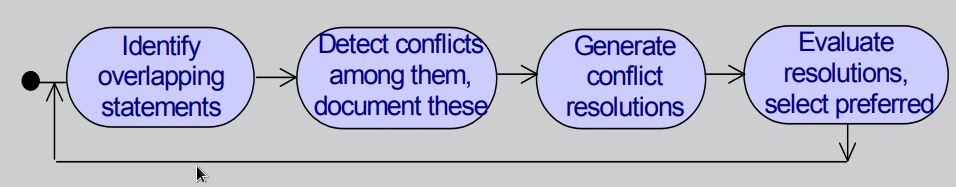
\includegraphics[width=0.9\textwidth]{images/managing_conflicts.png}
    \caption{چهار قدم چرخشی مدیریت تضاد‌ها}
\end{figure}

مدیریت تضاد‌های ضعیف و قوی در ۴ قدم انجام می‌شود:

\begin{enumerate}
    \item \lr{Identify overlapping statements}: شناسایی عباراتی که با هم مشترک
    هستند و در مورد یک مفهوم مشترک صحبت می‌کنند. شباهت‌ها می‌توانند فاعل، فعل و
    مفعول باشند. عملیاتی که در کنار یکدیگر دچار تضاد نمی‌شوند. \begin{enumerate}
        \item پدیده‌های باز و بسته شدن در‌های قطار مفاهیم رایج در سبد
        نیازمندی‌های آن است.
        \item پدیده‌های بدست آوردن کتاب، قرض گرفتن و بازگرداندن کتاب نیز از
        مفاهیم رایج مرتبط به \lr{Book copy} می‌باشد.
    \end{enumerate}
    \item \lr{Detect conflicts among them, document these}: از میان جملات
    جمع‌آوری شده باید بررسی کنیم که ببینیم چه نظراتی با هم همپوشانی دارند. اگر
    از میان همپوشانی‌ها تضادی پیدا شد بایستی تضاد‌ها را داکیومنت کنیم. راه‌های
    تشخیص تضاد: \begin{enumerate}
        \item \lr{Informally} یا غیررسمی: به صورت غیررسمی اعلام می‌کنیم که
        همپوشانی عبارات با هم رضایت بخش هستند و تحت چه شرایطی راضی کننده نیستند؟
        به گونه‌ای که به صورت چشمی منطقی نیستند.
        \item استفاده از روش‌های اکتشافی یا \lr{Heuristics} (استفاده از درخت):
        براساس یک جدول مشخص می‌کند که جملات چگونه می‌توانند با یکدیگر تضاد داشته
        باشند.
        \item استفاده از روش رسمی یا \lr{Formally}: تکنیک‌های اثبات قضیه. در
        حالت رسمی نرم‌افزار‌های بحرانی را نمی‌توان \lr{UML} کرد چرا که نیاز به
        اثبات دارند. نمایش و اعتبارسنجی هم با استفاده از زبان‌های رسمی امکان
        پذیر می‌باشد.
        \item استفاده از الگو‌های تضاد که نسخه‌ای سبک‌تر از تکنیک‌های رسمی
        هستند. نتیجه به صورت گرافیکال می‌باشد.
    \end{enumerate}
    \item \lr{Generate conflict resolutions}: رزولوشن یک مفهوم است که کتاب مرجع
    برای مدیریت تضاد از آن استفاده می‌کند. هر  راه‌حلی که به ذهن مهندس نیازمندی
    رسید باید کامل آن را بیان کند.
    \item \lr{Evaluate resolutions, select preferred}: باید یکی از راه‌حل‌هایی
    که در مرحله پیشین ارزیابی کردیم را بررسی کنیم و بهترین آنها را انتخاب کنیم.
\end{enumerate}

\subsubsection*{نکات}

\begin{itemize}
    \item همانطور که می‌دانیم \lr{Statements} سبد ما می‌باشد و راه‌حل‌هایی که
    بدست می‌آوریم باید از جنس سبد باشد. اولین راه‌حل \lr{Drop} کردن می‌باشد.
    همچنین از دیگر راه‌حل‌های تغییر جمله و سازگار کردن آن است، حتی ما می‌توانیم
    برای حل تضاد جمله به آن جمله‌ای مناسب را اضافه کنیم.
    \item مهندس نیازمندی باید در \lr{Intra-viewpoint}ها بازه را تعیین کند.
    \item برای رفع تضاد ممکن است جمله‌ای را حذف، اضافه یا حتی تغییر دهیم. در این
    حین ممکن است بازم ایجاد تضاد صورت گیرد به همین خاطر ۴ قدم مدیریت تضاد‌ها به
    صورت چرخشی می‌باشد.
    \item ما باید عواملی که با هم تضاد دارند را بشناسیم که بتوانیم آن‌ها را
    مدیریت کنیم.
    \item باید بدانیم که کدام موارد باعث ایجاد تضاد می‌شوند و بعد از تغییر سبد
    می‌توانند دردسرزا شوند.
    \item معمولاً \lr{Conflict}خیز‌ها در \lr{Overlap} های زیادی شرکت می‌کنند.
    \item جملاتی را باید استفاده کنیم که در \lr{Overlap}های زیادی شرکت داشتن و
    شرکتشان خوب و بدون تضاد بوده.
\end{itemize}

\subsection{تکنیک‌های داکیومنت کردن}

\begin{figure}[H]
    \centering
    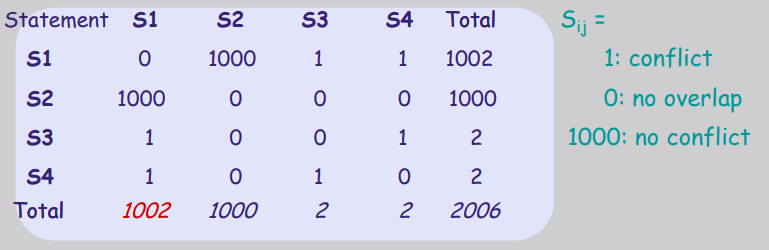
\includegraphics[width=0.9\textwidth]{images/systematic_process_table.png}
    \caption{تشخیص تضاد‌ها و همپوشانی‌ها}
\end{figure}

\subsubsection*{نکته}

\begin{itemize}
    \item باقی مانده نشان‌دهنده تضادهای بین دو جمله می‌باشد.
    \item خارج قسمت نشان‌دهنده همپوشانی مناسب و بدون تضاد است.
\end{itemize}

\begin{equation}
    Conflicts(S1) = remainderOf(1002/1000) \rightarrow 2
\end{equation}

\begin{equation}
    nonConflictingOverlaps(S1) = quotientOf(1002/1000) \rightarrow 1
\end{equation}

\begin{equation}
    Conflicts(Total) = remainderOf(2006/1000) \rightarrow 6
\end{equation}

\begin{equation}
    nonConflictOverlaps(Total) = quotientOf(2006/1000) \rightarrow 2
\end{equation}

\subsection{تکنیک‌های رفع تضاد}

برای رفع تضاد ۴ روش مطرح شده است که هر کدام از آن‌ها می‌توانند منجر به تولید
نیازمند‌های جدید شوند تا تضاد موجود در جمله را رفع کنند:

\subsubsection{خاص‌سازی منبع یا هدف تضاد}

تضاد در سطح جمله رخ می‌دهد، یعنی یک قانون به کل وارد می‌شود که یکسری جزئیات
دارد. نقض قانون بالایی به جز وارد می‌شود. هر کدام از جزئیات قوانین خودشان را
دارند و چون جز هم قانون خودش را دارد باعث ایجاد تضاد می‌شود. قانون جدید (جمله
جدید) در مورد کل سیستم نبوده و بلکه در مورد یک جز خاص می‌باشد. به جای اعمال
قانون به کل سیستم بایستی به یک نود و قشر مشخص این قانون جدید اعمال شود. معمولاً
در فاعل و مفعول رخ می‌دهد.

برای مثال:

\begin{itemize}
    \item به کاربران (\lr{Users}) اجازه داده شود که بتوانند از وضعیت کتابی که به
    امانت گرفته شده است مطلع شوند.
    \item دانشجویان نباید از وضعیت کتاب امانت گرفته شده مطلع باشند.
\end{itemize}

خاص‌سازی باید روی منبع یا رابطه کل به جز اعمال شود. در مثال بالا مشخص نیست که
کاربران دقیقاً چه قشری هستند و آیا شامل قشر دانشجویان می‌شود؟ پس بایستی قانونی
تعریف کنیم که مشخص شود چه گروهی قادر به مطلع شدن وضعیت باشند و چه گروهی
نمی‌توانند. به همین دلیل مجوز‌هایی برای \lr{Staff users} صادر می‌کنیم و مجوز
دیگری به نام \lr{Students}. در این دو گروه به روشنی می‌توان قابلیت‌هایشان را
شخصی‌سازی نمود. گروه خاص ما فاعل بوده است. چه کسانی بتوانند و چه کسانی نتوانند؟

\subsubsection{ضعیف‌تر کردن جملاتی که تضاد دارند}

در این روش معمولاً جمله سخت‌تر را ضعیف (\lr{Weak}) می‌کنیم. دقیقاً جزئی که قانون
را می‌بندد.

برای مثال:

\begin{itemize}
    \item پدر می‌گوید ساعت ۱۰ شب خانه باش اما مادر شما می‌گوید که هر چقدر بودی
    مشکلی نداره، در این جمله تضاد قوی را مشاهده خواهیم کرد.
    \item قرض گیرنده کتاب، باید کپی کتاب را سر مهلت سه هفته‌ای تحویل دهد مگر
    اینکه یک مجوز (\lr{Permision}) برای استفاده بیشتر کپی کتاب برای دانشجو صاد
    شود.
    \item مثال دقیق‌تر: دانشجو‌ها می‌توانند تا سه هفته کپی کتاب را از کتابخانه
    قرض بگیرند اما در صورتی که عضو انجمن علمی دانشگاه باشند می‌تواند ۵ هفته کتاب
    را داشته باشند.
\end{itemize}

\subsubsection{ری‌استور کردن}

در این روش تا زمانی که به تضاد بر نخورده‌ایم پیش می‌رویم و بعد از برخورد به تضاد
سیستم را به حالت قبل از تضاد خواهیم برد.

برای مثال دانشجو می‌خواهد کتاب را بیشتر از ۳ هفته قرض بگیرد، اما کتابخانه تنها ۳
هفته امکان قرض گرفتن را برای دانشجو فراهم کرده است. برای حل این تضاد کتابخانه از
ری‌استور کردن استفاده می‌کند و می‌گوید برای قرض گرفتن بیشتر از ۳ هفته، سر موعد
مهلت قرض گرفتن کتاب را تمدید کن.

\subsubsection{پرهیز از شرایط مرزی}

آخرین راه‌حل که سخت‌تر از بقیه می‌باشد این روش است که در مورد تضاد‌های ضعیف یا
(\lr{Weak conflict}) صادق خواهد بود. در این روش تلاش بر این است که شرایط مرزی را
برای تضاد‌ها به گونه‌ای کنترل کنیم که هیچ وقت رخ ندهند تا هدف سیستم را از بین
برود.

برای مثال، فرض کنید کتابخانه از یک کتاب مخصوص، تنها سه کپی دارد. اگر هر کدام از
این سه کپی را سه دانشجو مختلف قرض بگیرد، دانشجوی چهارم نمی‌تواند این کتاب را
درخواست کند. یعنی ریشه‌یابی یکسری کتاب که مرجع آن مشخص است که دیگر هیچ کپی از آن
در کتابخانه موجود نیست به این صورت رسماً رسالت کتابخانه زیر سوال رفته است. سوالی
که می‌تواند مطرح شود این است که آیا این نگرانی برای همه کتاب‌ها وجود دارد؟ باید
این مسئله بررسی گردد که برای چه کتاب‌هایی نیاز داریم شرط جدیدی را وضع کنیم. برای
کامل کردن مثال، فرض کنید از آن کتابی که در ابتدای فرضمان سه کپی داشتیم تنها دو
کپی قابل قرض دادن به دانشجو باشد و کپی آخر کتاب تنها زمانی قابل استفاده است که
خواننده کتاب درون کتابخانه باشد و نخواهد آن را به بیرون از کتابخانه ببرد.

برای مثال بالا ممکن است به دنبال الگوریتم‌های دسته‌بندی برویم که بتوانیم رضایت
را برای همه طرفین برقرار کنیم تا همه بتوانند از تمام کپی‌ها به صورت مناسب
استفاده کنند.

در شرایط مثال بالا سیستم کتابخانه بسیار اساسی‌تر خواهد شد و باید در صفات کلاس
مربوطه و نیازمندی‌ها خود اعلام کنیم که چند کپی از کتاب‌ها قابل قرض و چند کپی
قابل استفاده در محل کتابخانه می‌باشد.

\subsection{تمرین اول}

در یک سیستم مانند اسنپ، مسافر می‌خواهد نزدیک‌ترین ماشین به او تخصیص داده شود،
مدیر سیستم می‌خواهد در راستای طرح تشویقی خود رانندگانی با امتیاز بالاتر را به
مشتری تخصیص دهد. آیا تضادی می‌بینید؟ اگر بله از چه نوعی است و راه‌حل آن چیست؟

بله تضاد دارند، دو جمله وجود دارد:

\begin{itemize}
    \item کاربر به دنبال نزدیک‌ترین راننده اسنپ می‌باشد
    \item مدیر می‌خواهد راننده‌ای انتخاب شود که بالاترین امتیاز را داشته باشد.
    \item تضاد در جایی رخ می‌دهد که ممکن است راننده‌ای با امتیاز بالا در شعاع
    دورتری قرار داشته باشد.
    \item در این سناریو مشکلی برای راننده، مدیر و کاربر پیش نمی‌آید. پس تضاد
    ضعیف است. ما می‌توانیم با رویکرد \lr{Restore} کردن این تضاد را به گونه‌ای
    پوشش دهیم که همه راضی باشند.
    \item لزوماً امتیاز راننده می‌تواند ۵ ستاره اولین شعاع نزدیک به کاربر نباشد
    براساس درخواست کاربر مشخص می‌شود که کدام راننده با امتیاز بالا بایستی فیلتر
    شود و از بین آنها کدام راننده می‌خواهد درخواست کاربر را بپذیرد. این بدان
    معناست که درخواست کاربر برای رانندگانی که در همان شعاع هستند که امتیاز آن‌ها
    کم باشد، ارسال نمی‌شود.
\end{itemize}

\subsection{مدیریت ریسک}

معمولاً در فاز‌های اولیه یک پروژه نرم‌افزاری، مهندسان نیازمندی و ذینفعان
انتظارات عجیبی را دارند:

\begin{itemize}
    \item محیط و نرم‌افزار همانگونه که انتظار دارند رفتار کند.
    \item برنامه توسعه نرم‌افزاری پروژه همانگونه که برنامه‌ریزی شده است رو به جلو
    باشد.
\end{itemize}

اما در حقیقت جا به جایی از \lr{System-as-is} به \lr{Sysmte-to-be} ممکن است دچار
ریسک‌های مختلفی شود.

\subsubsection{شدت ریسک یا \lr{Severity}}

درجه از دست دادن رضایت نسبت به یک هدف را شدت ریسک یا \lr{Severity} می‌گویند.

ریسک‌ها نقض (\lr{Not}) یک نیاز می‌باشند. وقتی یک نیاز به درستی انجام نشود یا به
هر دلیلی دیر انجام شود و نقض یک جمله باشد می‌توان گفت که به ریسک تبدیل شده است.
نکته حائز اهمیت آن است که ریسک روی یک جمله می‌باشد و روی دو جمله مانند تضاد‌ها
تاثیر ندارد.

ریسک‌ها به دو دسته تقسیم می‌شوند:

\begin{enumerate}
    \item مرتبط با محصول یا \lr{Product-related}
    \item مرتبط با فرایند یا \lr{Process-related}
\end{enumerate}

\subsubsection{مرتبط با محصول یا \lr{Product-related}}

بیشترین ارتباط را به مهندس نیازمندی دارد. الزاماتی که در طراحی یک سیستم بایستی
در نظر گرفته شود تا بتوانیم سیستم را در برابر آن‌ها تجهیز کنیم؛ لذا افرادی در
حوزه مدیریت ریسک کار می‌کنند که متخصص آن دامنه و سیستم هستند. یعنی کاملاً در
مورد دامنه تجربه و اطلاعات مناسب را دارا هستند. این افراد معمولاً جایگاه‌های
ثابتی در دامنه خود داشتند. مانند سیستم‌های حسابداری بانکی، سیستم‌های \lr{CRM} و
غیره. تمام حالات سیستم را دیده‌اند و در استراتژی‌های مختلف در برابر ریسک‌های
مرتبط را تجربه کرده‌اند. به عبارتی ساده‌تر یعنی به طور کل این افراد شناخت بسیار
کاملی نسبت به آن دامنه دارند.

این ریسک‌ها می‌توانند مانند مثال‌های زیر باشند:

\begin{itemize}
    \item ریسک در برابر ارسال و دریافت اطلاعات داخل برنامه‌ای؛ پیامی که ارسال
    می‌شود و قرار است به یک نفر برسد ریسک موارد زیر را دارد: \begin{itemize}
        \item پیام برای آن شخص مشخص ارسال نشود و به تمام کاربران داخل شبکه بدون
        اجازه ارسال شود. (\lr{Broadcastly send})
        \item پیام با تاخیر در شبکه ارسال شود و به دست دریافت کننده پیام برسد.
        \item شبکه شنود شود و محتوای پیام را بتوان به صورت غیرقانونی در شبکه
        مشاهده نمود.
        \item پیام قابلیت ویرایش پس از ارسال را داشته باشد.
    \end{itemize}
    \item سیستم حاوی احراز هویت می‌باشد و ریسک آن: \begin{itemize}
        \item اگر کاربر گذرواژه خود را فراموش کرده باشد؟ پس بایستی استراتژی
        مناسب در برابر این ریسک را در نظر بگیریم و برای این سیستم احراز هویت
        گزینه فراموشی گذرواژه را طراحی کنیم.
    \end{itemize}
\end{itemize}

\subsubsection{مرتبط با فرایند یا \lr{Process-related}}

تمام اتفاقاتی که در ارتباط مستقیم با محصول نمی‌باشد را شامل می‌شود. برای مثال
ممکن است ارزش پولمان کم‌تر شود یا یکی از اعضا/پرسنل‌مان استعفا دهد.اینگونه
ریسک‌ها مرتبط با مدیر پروژه می‌باشد.

\subsection{چرخه مدیریت ریسک}

\begin{itemize}
    \item فرایند پیدا کردن ریسک در پروژه‌های نرم‌افزاری یک فرایند تکرارپذیر
    می‌باشد که شامل سه مرحله‌ زیر می‌باشد: \begin{enumerate}
    \item \lr{Risk identification}: شناسایی ریسک: دقیقاً ریسکی در سیستم به صورت
    مشخص رخ می‌دهد؟ یا اتفاق افتاده است؟
    \item \lr{Risk assessment}: ارزیابی ریسک: آیا عواقب احتمالی بدی دارد؟
    می‌توان از آن جلوگیری کرد؟ آیا می‌توان تاثیرات رخدادش را مدیریت و کنترل کرد؟
    \item \lr{Risk control}: کنترل ریسک: مدیریت و کنترل ریسک به عنوان نیازمندی
    جدید
\end{enumerate}
    \item در این میان نکته بسیار مهم آن است که در چرخه تکرار بررسی ریسک ممکن است
    هر عملیات و اقداماتی منجر به ایجاد ریسک جدیدی شود.
    \item مدیریت ضعیف ریسک‌ها عامل اصلی شکست در پروژه‌های نرم‌افزاری می‌باشد.
    \begin{enumerate}
        \item اشتباه فکر کردن به جریانات پروژه که انگار قرار نیست هیچ فرایندی
        مشکل داشته باشد.
        \item عدم شناسایی و دستکم گرفتن ریسک‌ها که باعث ناقص و ناکافی در نظر
        گرفتن نیازمندی‌ها در پروژه شود.
    \end{enumerate}
\end{itemize}

\subsection{شناسایی ریسک}

در این قسمت به چهار تکنیک شناسایی ریسک در پروژه‌های نرم‌افزاری می‌پردازیم:

\subsubsection{چک لیست‌های ریسک}

بررسی چک لیست‌های ریسک هم می‌تواند در مورد ریسک‌های محصول باشد و هم در مورد
فرایند‌ها. برای مثال حوزه مالی اولین حوزه‌ای نیست که قبلاً وجود نداشته باشد و
دقیقاً این اولین سیستمی باشد که از قابلیت‌های مالی استفاده می‌کند. در حقیقت این
حوزه از قبل چندین بار مورد استفاده قرار گرفته شده است و توسط متخصصان مختلفی مورد
آزمون و تلاش بسیاری بوده که توانسته به بیشتر چالش‌ها و ریسک‌های آن پاسخ دهند. به
این ترتیب می‌توانیم تمام ریسک‌های آن را از قبل تهیه کنیم و بتوانیم در سیستم خود
آن‌ها را بررسی کنیم که اگر برخی قابلیت‌ها منجر به تولید ریسک شد بتوانیم راهکاری
برای آن طراحی و پیاده‌سازی کنیم. در حقیقت یک لیست راهنما از پیش تعیین شده
می‌باشد.

برای سناریو زیر می‌توان تمام ریسک‌ها را از قبل پیشبینی کرد و لیستی از باید‌ها را
برای آن به شکل زیر بررسی می‌کنیم:

وقتی ارسال کننده پیام بخواهد پیامی را برای دریافت کننده‌ای ارسال کند ریسک‌های
احتمالی موارد زیر خواهد بود:

\begin{itemize}
    \item درگاه پیام تغییر کند: استفاده از رویکردی امن.
    \item پیام در شبکه شنود شود: رمزنگاری و استفاده از شبکه‌های توزیع شده.
    \item تاخیر در ارسال پیام: بررسی زیرساخت‌های شبکه‌ای و حتی الگوریتم‌های
    ارسال و دریافت پیام.
\end{itemize}

نکته: محصولات همگی مشخص هستند و فرایند‌های آن‌ها کاملاً عمومیت دارد.

\subsubsection{بازبینی مولفه‌ها}

مولفه‌ها مخصوص محصول می‌باشد؛ المان‌ها در حقیقت همان مولفه‌ها هستند. آدم‌ها،
نرم‌افزار‌های موجود و نرم‌افزار‌هایی که قرار است توسعه داده شود، تماماً المان
محسوب می‌شوند. برای مثال در سیستم قطار المان سرعت‌سنج را مورد بررسی قرار می‌دهیم
تا ریسک‌هایش را متوجه شویم:

\begin{itemize}
    \item آیا می‌تواند وظیفه‌اش را به درستی انجام ندهد؟ بله ممکن است. وظیفه‌ آن
    بررسی حرکت قطار و سرعت آن است. عوامل مختلفی وجود دارد که می‌تواند سبب درست
    کار نکردن و یا توقف کار کردن آن شود.
    \item اگر سرعت فیزیکی قطار با سرعت اندازه‌گیری شده برابر نباشد یعنی این
    دستگاه مشکلی دارد.
    \item یکی از ریسک‌ها آن است که در حین حرکت یکی از مسافر‌ها اقدام به خراب کرد
    دستگاه کند.
\end{itemize}

یا مثال اپلیکیشن‌های وب و موبایل:

\begin{itemize}
    \item اگر کاربر به اشتباه دستش روی گزینه پاک کردن بخورد جا به جا مورد انتخاب
    شده حذف شود یک ریسک در نظر گرفته می‌شود.
    \item برای این ریسک طراحی دیالوگ را می‌توان در نظر گرفت که از کاربر تایید مجدد
    برای انجام کار خودش گرفته شود.
    \item همچنین بعد از طراحی و پیاده‌سازی دیالوگ می‌توانیم در مورد پیاده‌سازی
    قابلیت لیست موارد پاک شده بپردازیم؛ یعنی سیستم را به گونه‌ای بنویسیم که
    قابلیت حذف آن به صورت \lr{Soft delete} باشد.
\end{itemize}

همه ریسک‌ها را نمی‌توان مدیریت کرد بلکه باید برخی از آنها پذیرفته شود. به همین
خاطر هر سیستمی بنا به مقدار آستانه تحمل خودش ریسک‌ها را می‌پذیرد. ریسک‌ها را
بررسی می‌کند اگر از مقدار آستانه کوچک‌تر بود مدیریتش را به کاربران می‌سپارد.
بارزترین مثال سیستم انتخاب واحد آموزشیار که به روشنی امکانات لود بالانس کردن
درخواست‌های کاربران زیاد را با پایین‌ترین کیفیت می‌تواند مدیریت کند. به خاطر
اینکه به کل سیستم صدمه‌ای وارد نمی‌کند، طراح سیستم از مدیریت این ریسک صرف‌نظر
می‌کند.

\subsubsection{تعریف عواقب یا \lr{Consequence}}

تمام عواقب \lr{Consequence} یک ریسک بایستی برآورد و بررسی شود. اگر نتوانیم یک
ریسک را مدیریت کنیم پس ممکن است رخ دهد. بعد از رخ دادن آن باید عواقب و تاثیرات
(\lr{Side effect}های) آن را در نظر بگیریم که چقدر می‌تواند مضر باشد و به سیستم
صدمه وارد کند. نوشتن تمام عواقب یک ریسک می‌تواند در کاهش نارضایتی‌ها تاثیرگذار
باشد.

\subsubsection*{آیا سیستم‌ها و سازمان‌ها از یک آستانه تحمل یکسان و مشخصی استفاده
می‌کنند؟}

خیر؛ هر سازمانی تحت شرایط و پروتکل‌های خاص خودش کار می‌کند و هر کسی نمی‌تواند
طبق میل و اراده خودش عمل کند. یک سازمان بررسی می‌کند که این مقدار آستانه چقدر
ارزش دارد.

پرسیدن چهار سوال زیر برای بررسی مولفه‌های ریسک الزامی می‌باشد؛ بایستی مولفه‌های
خیلی بزرگ را کوچک کنیم تا بتوانیم به سادگی به پاسخ سوالات زیر برسیم.

نکته: اینکه یک سناریو تبدیل به ریسک شود و به وقوع بپیوندد بایستی عواقب بعد از آن
را کنترل کنیم. مهندس نیازمندی لازم است که آثار ریسک را کمتر کند یا حداقل بتواند
آن‌ها را مدیریت کند. قدم‌های مدیریت ریسک متفاوت می‌باشد.

\begin{enumerate}
    \item \lr{Can it fall?} - آیا امکان رخ دادن همچین رسیکی وجود دارد؟ 
    \item \lr{How?} - بیشتر برای پیامد‌ها و بعد از درد رخ دادن ریسک است. 
    \item \lr{Why?} - چرا همچین ریسکی به وجود آمده است؟ دقیقاً به ریسک اشاره
    دارد.
    \item \lr{What are possible consequences?} - پیامد و عواقبی که ممکن است به
    همراه داشته باشد چه مواردی هستند؟ آیا از آن‌ها می‌توان چشم‌پوشی کرد؟ یا
    بایستی برای رفع آن‌ها هزینه‌ای داشته باشیم و راهکاری مناسب را ارائه دهیم؟
\end{enumerate}

\subsubsection{درخت ریسک}

به جزئیات این تکنیک در فصل نهم بیشتر پرداخته می‌شود.

تمام نود‌های درخت ریسک‌ها هستند. از ریشه شروع می‌کنیم و به ریسک‌های کوچک‌تر
شکسته می‌شود. برای مثال:

\begin{itemize}
    \item اگر خانه آتش بگیرد: \begin{enumerate}
        \item انفجار گاز
        \item اتصالی سیم برق داخل ساختمان
        \item یعنی یک اتفاق بزرگ و بد (آتش گرفتن یک خانه) می‌تواند چند عامل کوچک
        در رخ دادن آن تاثیر داشته باشند.
    \end{enumerate}
\end{itemize}

\subsubsection*{چه زمانی نیامند کشیدن درخت ریسک هستیم؟}

زمانی که ریسک به اندازه‌ای بزرگ و پیچیده باشد که نتوانیم آن را بفهمیم و درک
کنیم، نیازمند آن هستیم که با استفاده از درخت ریسک، یک ریسک را به عوامل مهم و
تاثیرگذارش بشکنیم تا ببینیم می‌توانیم آن را کنترل کنیم یا با سطح آستانه تحمل
سیستم ما حل خواهد شد.

\subsubsection*{نکات}

\begin{itemize}
    \item در این بین بعضی از معیار‌هایی که در درخت مشخص می‌کنیم ممکن است به صورت
    آماری باشند؛ یعنی طی ۵۰ سال مثلاً دوبار خانه آتش گرفته است.
    \item در تمام صنایع ریسک وجود دارد.
    \item ریسک‌ها را یا با مستطیل نمایش می‌دهیم یا با بیضی.
    \item اگر ریسک نیاز به شکستن داشته باشد آن را با نماد مستطیل نمایش می‌دهیم.
    \item اگر به کوچک‌ترین حالت ریسک رسیده باشیم یعنی آن را بتوانیم کامل به
    ساده‌ترین روش درک کنیم و نیاز به شکست نداشته باشد از نماد بیضی استفاده
    می‌کنیم.
    \item نماد‌های دیگری مانند \lr{AND} و \lr{OR} در این درخت استفاده می‌شوند.
    \item برگ‌ها و نود‌های پایانی درخت همیشه با نماد بیضی نمایش داده می‌شوند.
    \item برای آنکه پیدا کردن ریشه اتفاقاتی که رخ می‌دهد، ساده‌تر باشد از درخت
    ریسک استفاده می‌کنیم تا بتوانیم اتفاق بالایی را شناسایی کنیم و سپس بعد از آن
    با الگوریتم \lr{Cutset} درخت را ساده‌تر می‌کنیم.
    \item میزان بزرگی توپ، بزرگی خطر را نشان نمی‌دهد.
    \item پارامتر دیگر در بررسی بزرگی توپ ریسک احتمال وقوع هر عاقبت می‌باشد.
    \item اول عواقب پیدا می‌شود و سپس احتمال هر عاقبت سنجیده می‌شود.
    \item احتمال وقوع ریسک اگر کم باشد نمی‌توانیم بگوییم که میزانش نیز کمتر بوده
    است.
    \item احتمال وقوع ممکن است کم باشد اما اگر رخ بدهد ممکن است سیستم را از کار
    خارج کند.
\end{itemize}

\subsubsection{فلسفه درد}

درد صفر شدنی نیست اما قابل کم شدن است. چون اگر عواقب هم مورد بررسی قرار گیرد
می‌تواند درد داشته باشد؛ اگر درد نداشته باشد باید شک کنیم که آیا ریسک روی سیستم
ما رخ داده است؟ یا روی سیستم دیگری بوده؟ جعبه کمک‌های اولیه بهبود و کاهش اثر
اتفاقاتی است که مدتی است که رخ داده.

\subsubsection{نکات گره‌های \lr{AND} و \lr{OR}}

دقیقاً همانند مدار منطقی عملگر‌های زیر به این شکل کار می‌کند:

\begin{itemize}
    \item نود \lr{AND}: تمام زیر نود‌ها بایستی اتفاق بیوفتند تا نود والد رخ دهد.
    \item نود \lr{OR}: تنها نیاز است یک نود رخ دهد تا اتفاق والد رخ دهد.
\end{itemize}

\begin{figure}[H]
    \centering
    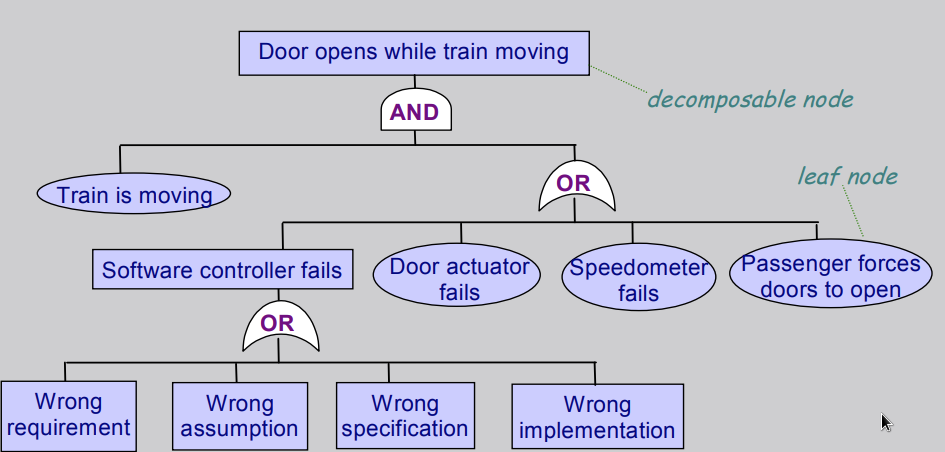
\includegraphics[width=0.9\textwidth]{images/risk_tree_sample.png}
    \caption{درخت ریسک از مسئله قطار}
\end{figure}

\subsubsection{شرط‌های \lr{Cutset}}

\begin{itemize}
    \item اگر از نوع \lr{AND} باشد یک نود درست شود و هر چیزی که به آن وصل بود را
    به آن منتقل می‌کنیم.
    \item اگر از نوع \lr{OR} بود به ازای هر نود مقایسه \lr{OR} صورت می‌گیرد.
\end{itemize}

\begin{figure}[H]
    \centering
    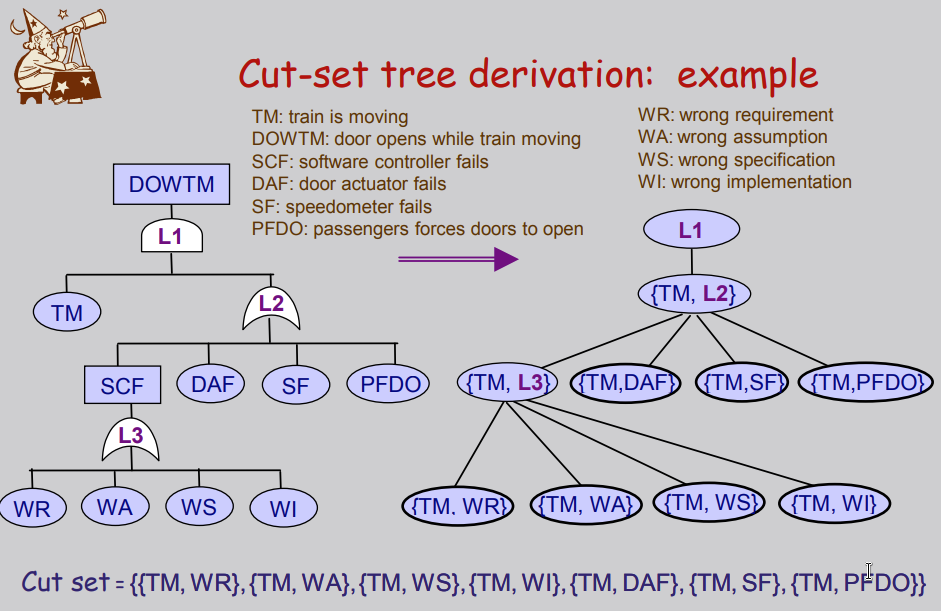
\includegraphics[width=0.9\textwidth]{images/cutset_risk_tree.png}
    \caption{ساده‌سازی درخت ریسک}
\end{figure}

\subsubsection{استفاده از تکنیک‌های جمع‌آوری داده}

با افراد و آدم‌ها در ارتباط می‌باشد. کسانی که ذینفع هستند در قسمت استخراج
اطلاعات می‌توانند نقش پر رنگی را ایفا کنند. اگر از متخصصین این حوزه سوال بپرسیم
می‌توانیم رخداد‌ها و پیامد‌های مختلفی که می‌تواند یک ریسک داشته باشد را یاد
بگیریم. مهم‌ترین راه‌ها: مانند استفاده از روش \lr{Interview} و روش \lr{Group
session}.

نکته: همان‌گونه که راه‌حل رفع تضاد رزولوشن بود، برای حل و کنترل ریسک از اقداماتی
مخصوص استفاده می‌کنیم تا بتوانیم به نسبت متعادلی ریسک را کنترل کنیم و حتی آن را
رفع کنیم (استفاده از تکنیک‌های \lr{Countermeasures} که در بالاتر گفته شد).

در این روش ابتدا راه‌حل را ارزیابی می‌کنیم و سپس بهترین راه‌حل را نسبت به بقیه
انتخاب و در سیستم در حال طراحی (\lr{System-to-be}) استفاده می‌کنیم.

\subsection{ارزیابی ریسک یا \lr{Risk assessment}}

هدف اصلی از ارزیابی ریسک، ارزیابی احتمال خطر + شدت، احتمال عواقب برای کنترل
خطرات بالا با اولویت بالا می‌باشد.

متغیر‌هایی که می‌توانیم برای ارزیابی کیفی مورد استفاده قرار دهیم:

\begin{itemize}
    \item برای احتمالات: (بسیار محتمل، محتمل، ممکن، بعید و...)
    \item برای شدت: (فاجعه‌بار \footnote{\lr{Catastrophic}}، شدید
    \footnote{\lr{Severe}}، بالا، متوسط و....)
\end{itemize}

\subsubsection*{چند عدد بزرگی ریسک را می‌سازند؟}

احتمال وقوع ریسک:

\begin{equation}
    P_{r} \epsilon (0, 1) \rightarrow 1 (State)
\end{equation}

احتمال وقوع عواقب:

\begin{equation}
    P_{c1} \epsilon (0, 1) P_{c2} \cdots \rightarrow n (State)
\end{equation}

شدت و دردی که در سیستم پس از عواقب پدیدار می‌شود:

\begin{equation}
    S_{c1} \{1, 2, 3, 4, 5\} S_{c1} \cdots \rightarrow n (State)
\end{equation}

اعدادی که بزرگی ریسک را می‌سازند (بزرگی توپ ریسک را می‌سازد):

\begin{equation}
    2n + 1
\end{equation}

سوال مهم آن است که چگونه می‌توان این اعداد را با هم ترکیب کرد که میزان خطر ریسک
را پیدا کرد؟ عواملی که مورد بررسی قرار گرفته است از یک جنس نیستند که بتوانیم
آن‌ها را با یکدیگر ترکیب کنیم.

\subsubsection{محاسبه میزان خطر ریسک}

\begin{equation}
    EX\footnote{\lr{Exposure}: نشان‌داده شدن}(r) = \sum_{i = 1}^{n} P_{c_{i}} \times S_{c_{i}}
\end{equation}

متغیر‌ها:

\begin{enumerate}
    \item n تعداد عاقبت
    \item P احتمال رخداد
    \item c \lr{Consequence}
    \item S \lr{Severity}
\end{enumerate}

اگر $n = 3$ باشد آنگاه میزان ریسک با توجه به محاسبات انجام شده بالا به شکل زیر
حاصل می‌شود:

\begin{itemize}
    \item $n = 3$
    \item $max = 15$: که از طریق محاسبات شماره ۱۵ و ۱۷ بدست آمده است.
    \item $min = 0$
\end{itemize}

فرض شود مقدار \lr{EX} برابر با ۷ شده است:

\begin{equation}
    EX = \frac{EX - min}{max - min} = \frac{7 - 0}{15 - 0} = \frac{7}{15}
\end{equation}

عدد $\frac{7}{15}$ میزان خطر ریسک بدست آماده می‌باشد که از طریق آن می‌توان
مقایسه‌ای بین آستانه تحمل درد دامنه خود کنیم که تا چقدر می‌تواند این ریسک برای
سازمان تاثیرگذار باشد.

\begin{equation}
    EX \epsilon [0, 15]
\end{equation}

\subsubsection{راه‌حل‌های ریسک}

راه‌حل‌های رفع ریسک پنج مورد می‌باشد:

\begin{enumerate}
    \item $P_{r} \searrow$: یا احتمال وقوع ریسک را کم می‌کنیم.
    \item $P_{r} = 0$: یا احتماع وقوع ریسک را صفر می‌کنیم. با طراحی که در حال
    انجام هستیم ریسک‌ها را شناسایی کرده‌ایم و می‌توانیم احتمال وقوع آن‌ها را به
    صفر برسانیم. مانند \lr{Iran access} کردن شبکه یک سرور در حالی که از شبکه
    خارج مورد حمله قرار گرفته بود. در این رویکرد اصلاً دیگر نمی‌تواند از شبکه
    خارجی حمله‌ای صورت گیرد.
    \item $P_{c_{i}} \searrow$: احتمال وقوع عواقب را کنترل می‌کنیم و آن را کاهش
    می‌دهیم. تمام سرویس‌های مورد نظر را از سرور آلوده به سرور دیگر در شبکه داخلی
    منتقل می‌کنیم. دکتر مقیم در قطار برای کاهش تاثیر ریسک و مدیریت عواقب می‌باشد.
    \item $P_{c_{i}} = 0$: احتمال وقوع عواقب را صفر می‌کنیم. بعد از آلوده شدن
    سرور، برق کل دیتاسنتر را قطع می‌کنیم که حمله به سرور‌های دیگر رخ ندهد (به
    عنوان مثال غیرحرفه‌ای).
    \item $S_{c_{i}} \searrow$: درد صفر شدنی نیست کم شدنی است.
\end{enumerate}

\subsubsection*{نکات}

\begin{itemize}
    \item در این راه‌حل‌ها، هر لایه که جلوتر می‌رویم لایه قبلی رخ داده است که
    بتوانیم ادامه ریسک‌ها را مدیریت و کنترل کنیم.
    \item برای بررسی ریسک‌ها بین صفر کردن و کم کردن احتمال هر کدام، از عبارت
    «یا» استفاده خواهیم کرد. یا باید ریسک صفر شود یا اگر نتوانستیم ریسک را صفر
    کنیم آن را حداقل کنترل و کم‌تر کنیم.
    \item دید مهندس نیازمندی نسبت به ریسک بسیار مهم است. ریسکی که می‌توان صفر
    کرد دیگر نیازی نیست که استراتژی برای کم کردن احتمالش را در نظر بگیریم.
    \item اگر سه لایه را بررسی کنیم، ممکن است با در نظر گرفتن استراتژی‌هایی مشکل
    را در همان لایه اول یا دوم حل کرده باشیم پس لزومی ندارد که تمام لایه‌ها را
    بررسی و برای آن‌ها استراتژی مناسب را در نظر بگیریم.
    \item ممکن است برای لایه‌ای از ریسک اصلاً راه‌حلی نداشته باشیم.
\end{itemize}

\subsubsection{مثال راه‌حل‌های ریسک}

\subsubsection*{مثال ۱}

\begin{itemize}
    \item \textbf{اتفاق بد محتمل این است که راننده قطار در هنگام حرکت به خواب
    برود. یک راه‌حل برای صفر کردن احتمال وقوع این ریسک ارائه دهید.} پیاده‌سازی
    قابلیت حرکت و مسیریابی خودکار یا \lr{Autopilot} بر روی قطا‌ر‌ها؛ با این
    نرم‌افزار می‌توان کنترل قطار را از انسان به سیستم انتقال داد و در صورتی که
    راننده احساس خستگی کرد می‌تواند بر روی حرکت قطار نظارت داشته باشد. به این
    شکل احتمال تصادف قطار را به دلیل خواب راننده آن صفر کرده‌ایم. استفاده از
    راننده قطار کمکی در سفر احتمال ریسک را کمتر می‌کند چرا که کمک راننده نیز
    می‌تواند احساس خستگی کند.
    \item \textbf{یک راه‌حل برای احتمال وقوع عاقبت این ریسک را بیان کنید که صفر
    کننده آن باشد.} وقتی در مورد عاقبت این ریسک صحبت می‌کنیم در حقیقت نه
    نرم‌افزار \lr{Autopilot} در قطار پیاده‌سازی شده است و نه راننده توانسته
    خستگی خود را کنترل کند و این بدان معناست که راننده در هنگام رانندگی قطار به
    خواب رفته است. برای این منظور می‌توانیم نرم‌افزاری از نوع \lr{AI} طراحی کنیم
    که اگر متوجه خوابیدن (بسته شدن چشم‌های راننده) در هنگام حرکت قطار شد، اعلانی
    به تمام مراکز و دیگر قطار‌ها ارسال کند که از حرکت خودشان منصرف شوند تا باعث
    برخورد دو قطار به یکدیگر نشوند و همچنین می‌توانند خطوط ریل را به گونه‌ای
    طراحی کنند که بعد از اعلان به این مراکز قطار را از طریق ریل‌ها نگه دارند و
    ماموری را برای جریمه راننده قطار ارسال کنیم تا از هر گونه تصادف در آینده
    جلوگیری کند.
    \item \textbf{راننده به خواب رفته است، خوابیدن راننده باعث برخورد دو قطار به
    یکدیگر شده است یعنی در حالت عواقب باز هم ریسک را کنترل نکرده‌ایم و حالا در
    مرحله درد یا \lr{Severity} هستیم.} در هر ۱۰ کیلومتر مسیر سازمان‌ها و
    بیمارستان‌های مجهز طراحی و پیاده‌سازی شوند که به سریع‌ترین حالت ممکن برای
    نجات جان مسافران دو قطار حاضر شوند. درون هر قطار، چند پزشک به همراه تجهیزات
    کامل در نظر گرفته شود که در هنگام تصادف در صورت امکان به آسیب دیدگان کمک
    کنند تا آن‌ها را به بیمارستان نزدیک برسانند. بعد از تصادف در‌ها و پنجره‌های
    قطار باز شوند که مسافرانی که جان آن‌ها سالم است بتوانند به خارج از قطار
    بروند و از هر احتمال انفجار و از بین رفتن جان‌ها جلوگیری شود.
\end{itemize}

\subsubsection*{مثال ۲}

تعریف ریسک: دانشجو نتواند وارد سیستم \lr{LMS} شود.

\begin{itemize}
    \item \textbf{کم کردن احتمال وقوع ریسک}: تعریف چندین سرور جانبی برای ورود
    موفقیت آمیز به کلاس‌ها.
    \item \textbf{دانشجو از طریق سرو‌ر‌های جانبی نتوانست وارد کلاس شود و الان در
    وضعیت ریسک در عاقبت هستیم}: قید و قانونی را می‌توانیم برای شروع هر کلاس وضع
    کنیم که اساتید ۱۵ دقیقه اول کلاس را به دور مباحث قبلی بپردازند یا اساتید دو
    بار حضور و غیاب را انجام دهند. همچنین می‌توان الگوریتمی را توسعه داد که به
    مدت زمان حضور دانشجو در کلاس می‌پردازد و حضور و غیاب توسط آن شکل می‌گیرد.
    \item \textbf{در لایه سوم، نه توانستیم احتمال وقوع را کنترل کنیم و نه در
    عاقبت توانستیم حاضر شویم. نوبت آن است که درد را برای دانشجو کمتر کنیم}: کلاس
    توسط اساتید در سامانه ضبط می‌شوند و دانشجو در صورت عدم حضور موفق در کلاس
    می‌تواند به کلاس ضبط شده مراجعه کند و از درس خود عقب نیوفتد.
\end{itemize}

به غیر از پنج تکنیکی که برای کنترل ریسک در بالاتر بررسی کردیم، استفاده از
تکنیک‌های جمع‌آوری اطلاعات از طریق ذینفعان می‌تواند کمک دیگری در فرایند بررسی
ریسک برای مهندسی نیازمندی باشد. استفاده از افراد خبره (\lr{Expert}) در این زمینه
می‌تواند به ما کمک کند که تمام چالش‌های پیاده‌سازی را بررسی کنیم و برای هر کدام
از آن‌ها از الگو‌های مطرح شده در سیستم‌های پیشین استفاده کنیم. تجربه‌های قبلی به
ما در کامل شدن سیستم و کمتر شدن ریسک‌های سیستمی کمک می‌کنند. برای مثال دو تیک
خوردن پیام در پیا‌مرسان‌های امروزی یک الگو برای مطمئن شدن از ارسال موفقیت آمیز و
خواندن شدن پیام توسط مخاطب و مقصد می‌باشد. فرقی نمی‌کند که این الگو‌ها برای
محصول باشد یا برای فرایند، دلیل آن که تمام سیستم‌های شبیه به یکدیگر هستند آن است
که یکسری از الگو‌های آن‌ها استاندارد و جامع می‌باشند.

نکته جالب دقیقاً از آن جایی است که الگو‌ها نیز می‌توانند در سیستم حاوی ریسک
باشند. برای مثال در گذشته که رمز پویا وجود نداشت افراد با استفاده از رمز دوم در
حساب بانکی خود می‌توانستند خرید خود را انجام دهند. اما تنها استفاده از رمز دوم
برای کاربر ایمن نمی‌باشد، پس استفاده از الگوی رمز‌های داینامیک یا پویا مطرح شد و
تمام بانک‌ها به این الگو پیوستند. در نظر داشته باشید اگر سرور کند شود و پیام رمز
پویا برای کاربر ارسال نشود در حقیقت ریسکی را برای کاربر ایجاد کرده‌ایم که برای
خرید و پرداخت وجه با مشکل رو به رو شده است. درست است که این الگو می‌تواند حاوی
ریسک باشد ولی از آنجایی که برای ما امنیت در اولویت است می‌توانیم از این ریسک چشم
پوشی کنیم و کاربر را وادار به صبر کردن و طراحی دکمه‌ای به نام "ارسال مجدد رمز"
کنیم.

\subsection{انتخاب راه‌حل مناسب برای رفع و کنترل ریسک}

بعد از آن که ریسک‌های سیستم مورد نظر را مهندس نیازمندی برآورد کرد ممکن است برای
کنترل یک ریسک به چندین راه‌حل مختلف برسیم. با چه معیار یا معیار‌هایی می‌توانیم
متوجه شویم که کدام راه‌حل برای کنترل ریسک مناسب است؟ دو روش برای انتخاب راه‌حل
ریسک مطرح شده است که میزان خوب بودن راه‌حل را برای کنترل ریسک مشخص می‌کند.

\subsubsection{اقدامات}

\lr{Countermeasure} به راه‌حل و اقدامات در برابر ریسک‌ها گفته می‌شود.

\subsubsection{ریسک‌ها بایستی مستند شوند}

برای توضیح نیازمندی راه‌حل‌های مطرح شده در کنترل ریسک‌ها، در ارزیابی سیستم
بایستی سندی در این رابطه تهیه شود. برای هر ریسک باید موارد زیر مشخص شود:

\begin{enumerate}
    \item شروط و رخداد‌هایی که باعث اتفاق افتادن ریسک می‌شوند.
    \item تخمین احتمال رخداد ریسک
    \item موارد محتمل و عواقب آن‌ها
    \item تخمین احتمال در وقوع ریسک، عواقب و درد‌های ناشی از آن‌ها
    \item مشخص کردن راه‌حل‌ها و اقدامات متقابل با ریسک‌ها در جهت کاهش ریسک
    \item انتخاب راه‌حل مناسب با استفاده از روش‌های بررسی آن‌ها
\end{enumerate}

\subsubsection{جنبه‌های استفاده از معیار‌ها}

استفاده از هر معیار دیگری میزان درگیری موارد زیر را متناسب با ریسک در بر دارد:

\begin{enumerate}
    \item میزان تاثیر راه‌حل در هزینه‌ها (\lr{Cost-effectiveness})
    \item میزان تاثیر راه‌حل در ریسک‌های دیگر
    \item میزان تاثیر راه‌حل در \lr{NFR}ها (مانند امنیت یا \lr{QoS})
\end{enumerate}

نکته: راه‌حل دادن باعث کوچک‌تر شدن توپ تاثیر می‌شود. همچنین اگر یک راه‌حلی مطرح
شود که در کوچک کردن چند توپ ریسک نقش داشته باشد می‌تواند کارآمد و الگو پذیر باشد
تا بتوانیم با مجموعه‌ای از راه‌حل‌ها به اندازه‌ای کمتر از آستانه مورد نظر خود
برسیم.

\subsubsection{روش \lr{RRL}}

\begin{equation}
    RRL(r, cm) = (Exp(r) - Exp(r/cm))/cost(cm)
\end{equation}

\begin{LTR}
    \begin{itemize}
        \item \lr{EXP(r)}: Exposure of rist r
        \item \lr{EXP(r/cm)}: New exposure of r if countermeasure cm is selected
    \end{itemize}
\end{LTR}

\begin{enumerate}
    \item در این روش راه‌حلی انتخاب می‌شود که بیشترین \lr{RRL}\footnote{\lr{Risk
    Reduction Leverage}} را داشته باشد
    \item .در این فرمول صورت کسر \lr{Effectiveness} بودن را مشخص می‌کند و در
    مخرج هزینه‌ها مشخص شده است.
    \item مقدار \lr{RRL} بیشتر باشد یعنی هزینه‌های آن را کاهش داده‌اند (مخرج
    کوچک‌تر اثر بخشی صورت را بیشتر نشان می‌دهد).
    \item روش \lr{RRL} نقش یک راه‌حل را در تمام ریسک‌ها بررسی نمی‌کند.
    \item این روش تنها در راه‌حل‌های تکی کار می‌کند. ما باید بررسی کنیم که یک
    راه‌حل در چند ریسک تاثیرگذار است.
    \item تمام راه‌حل‌ها را تک به تک بررسی می‌کند.
    \item تک به تک دیدن راه‌حل‌ها نسبت به ریسک‌ها در این روش باعث می‌شود که بعضی
    چیز‌ها در نظر گرفته نشود.
    \item یک فرض غلطی را دارد که می‌گوید یک ریسک را می‌توان با یک راه‌حل کنترل
    کرد. در حالی اگر یک راه‌حلی وجود داشته باشد که در کنترل چندین ریسک نقش داشته
    باشد بسیار ارزشمند‌تر از آن است که یک ریسک را با چندین راه‌حل مدیریت کنیم.
    \item $1(Risk) \rightarrow n(CM)$: روش مناسبی نخواهد بود.
\end{enumerate}

\subsubsection{روش \lr{DDP}}

این روش \footnote{\lr{Defect Detection Prevention}} هم نیز مانند روش \lr{RRL} به
صورت معیاری برای بررسی مناسب بودن راه‌حل برای کنترل ریسک می‌باشد با این تفاوت که
راه‌حل‌ها نسبت به ریسک‌ها به صورت تک به تک عنوان نمی‌شود و این روش به صورت
\lr{Generalization} عمل خواهد کرد. تکنیک و ابزاری است که در سال ۲۰۰۳ توسط ناسا
توسعه داده شده است.

\subsubsection*{تعاریف در این روش}

\begin{LTR}
    \begin{itemize}
        \item \lr{Objective} $\rightarrow$ \lr{requirement}
        \item \lr{Risk} $\rightarrow$ \lr{failure mode}
        \item \lr{Countermeasure} $\rightarrow$ \lr{PACT}
    \end{itemize}
\end{LTR}

برای انجام روش \lr{DDP} بایستی سه مرحله را طی کنیم:

\begin{enumerate}
    \item محاسبه ماتریس تاثیر ریسک به صورت دقیق
    \item محاسبه ماتریس تاثیر راه‌حل بر روی ریسک مورد نظر به صورت دقیق
    \item تعیین تعادل بهینه ریسک نسبت به هدف با تقسیم کاهش ریسک بر روی هزینه
    اجرای راه‌حل ($\frac{risk Reduction}{countermeasure cost}$)
\end{enumerate}

\subsubsection{مرحله اول در \lr{DDP}}

برای مرحله اول که رسم جدول تاثیر-نتیجه (جدول شماره \ref{fig:impactMatrix}) ریسک
می‌باشد باید در نظر داشته باشیم که هدف، موارد زیر می‌باشد:

\begin{itemize}
    \item اولویت‌بندی ریسک‌ها براساس امتیاز \lr{Critical impact} نسبت به تمام
    اهداف
    \item هایلایت کردن و برجسته کردن ریسک‌پذیر‌ترین اهداف
\end{itemize}

\subsubsection*{نکات}

\begin{itemize}
    \item تمام اعداد داخل جدول اعم از وزن‌ برای ریسک‌ها و اهداف و همچنین میزان
    تاثیرات، توسط اسناد قبلی در دامین و افراد خبره بدست آمده است!
    \item تلاقی سطر و ستون تاثیر ریسک روی هدف را نشان می‌دهد ($Impact(r, obj)$)
    \item اگر تاثیر ریسک صفر باشد یعنی هیچ تاثیری در هدف نداشته است.
    \item اگر تاثیر ریسک یک باشد یعنی به هدف تاثیر گذاشته است و ممکن است آن ریسک
    هدف را از بین ببرد.
    \item فرمول بدست آوردن آخرین سطر جدول: $Criticality(r) = Likelihood(r) * \sum_{obj}(Impact(r, obj) * weight(obj))$
    \item فرمول به دست آوردن آخرین ستون از جدول: $Loss(obj) = weight(obj) * \sum_{r}(Impact(r, obj) * Likelihood(r))$
    \item نتیجه \lr{Risk criticality} دردسر کل ریسک را بر اهداف نشان می‌دهد.
\end{itemize}

\begin{LTR}
    \begin{table}[H]
        \centering
        \begin{tabular}{ccccccc}
            Objectives & \makecell{Late returns \\ weight: \lr{0.7}} & \makecell{Stolen copies \\ weight: \lr{0.3}} & \makecell{Lost copies \\ weight: \lr{0.1}} & \makecell{LongLoan by staff \\ weight: \lr{0.5}} & Loss obj \\ \hline
            \makecell{Regular avialability of \\ book copies weight: \lr{0.4}} & \lr{0.30} & \lr{0.60} & \lr{0.60} & \lr{0.20} & \lr{0.22} \\ \hline
            \makecell{Comprehensive library \\ coverage weight: \lr{0.3}} & \lr{0} & \lr{0.20} & \lr{0.20} & \lr{0} & \lr{0.02} \\ \hline
            \makecell{Staff load reduced \\ weight: \lr{0.1}} & \lr{0.30} & \lr{0.50} & \lr{0.40} & \lr{0.10} & \lr{0.04} \\ \hline
            \makecell{Operational costs \\ decreased weight: \lr{0.2}} & \lr{0.10} & \lr{0.30} & \lr{0.30} & \lr{0.10} & \lr{0.05} \\ \hline
            Risk criticality & \lr{0.12} & \lr{0.12} & \lr{0.04} & \lr{0.06} &  \\
        \end{tabular}
        \caption{Impact matrix - example for library system}
        \label{fig:impactMatrix}
    \end{table}
\end{LTR}

\subsubsection{مرحله دوم \lr{DDP}}

برای مرحله دوم نیازمند رسم جدول تاثیر-نتیجه (جدول شماره
\ref{fig:effectivenessMatrix}) هستیم که هدف موارد زیر می‌باشد:

\begin{itemize}
    \item تخمین کاهش ریسک به وسیله راه‌حل جایگزین
    \item برجسته‌سازی بیشترین تاثیر راه‌حل‌های مطرح شده.
\end{itemize}

\subsubsection*{نکات}

\begin{itemize}
    \item تمام اعداد داخل جدول اعم از وزن‌ برای ریسک‌ها و اهداف و همچنین میزان
    تاثیرات راه‌حل، توسط اسناد قبلی در دامین و افراد خبره بدست آمده است!
\end{itemize}

\begin{itemize}
    \item تلاقی سطر و ستون کاهش و حذف ریسک را نشان می‌دهد اگر راه‌حل اعمال شده
    باشد $Reduction(cm, r)$.
    \item اگر مقدار صفر باشد یعنی راه‌حل پیشنهادی هیچ تاثیر نداشته است.
    \item اگر مقدار ۱ باشد یعنی به طور کامل از وقوع ریسک پرهیز کرده است.
    \item فرمول بدست آوردن آخرین سطر جدول به ازای هر ریسک: $combinedReduction(r) = 1 - \prod_{cm}(1 - Reduction(cm, r))$
    \item فرمول بدست آوردن آخرین ستون جدول به ازای هر راه‌حل: $overallEffect(cm) = \sum_{r}(Reduction(cm, r) * Criticality(r))$
    \item نتیجه \lr{Overall effect of countermeasure} مشخص می‌کند که این راه‌حل
    چقدر خوب بوده است.
    \item احتمال وقوع ریسک برایمان اهمیتی ندارد اما به هر دلیلی اینکه آن ریسک
    چقدر برایمان دردسرساز بوده، خیلی اهمیت دارد.
    \item در این مرحله به شما ثابت شد که بر خلاف روش \lr{RRL} یک راه‌حل می‌تواند
    در کاهش چند ریسک تاثیرگذار باشد. پس این راه‌حل ارزشمند است.
\end{itemize}

\begin{LTR}
    \begin{table}[H]
        \centering
        \begin{tabular}{ccccccc}
            Countermeasure & \makecell{Late returns \\ weight: \lr{0.7}} & \makecell{Stolen copies \\ weight: \lr{0.3}} & \makecell{Lost copies \\ weight: \lr{0.1}} & \makecell{LongLoan by staff \\ weight: \lr{0.5}} & \makecell{Overall effect of \\ countermeasure} \\ \hline
            \makecell{Email reminder sent} & \lr{0.70} & \lr{0} & \lr{0.10} & \lr{0.60} & \lr{0.12} \\ \hline
            \makecell{Fine subtracted from \\ registration deposit} & \lr{0.80} & \lr{0} & \lr{0.60} & \lr{0} & \lr{0.12} \\ \hline
            \makecell{Borrower unregistration \\ + insertion on black list} & \lr{0.90} & \lr{0.20} & \lr{0.80} & \lr{0} & \lr{0.16} \\ \hline
            \makecell{Anti-theft device} & \lr{0} & \lr{1} & \lr{0} & \lr{0} & \lr{0.12} \\ \hline
            \makecell{Combined risk \\ reduction} & \lr{0.99} & \lr{1} & \lr{0.93} & \lr{0.60} &  \\
        \end{tabular}
        \caption{Effectiveness matrix - example for library system}
        \label{fig:effectivenessMatrix}
    \end{table}
\end{LTR}

\subsubsection{مرحله سوم \lr{DDP}}

در مرحله پایانی به تعیین تعادل بهینه بین عامل کاهش‌دهنده ریسک و هزینه راه‌حل‌ می‌پردازیم.

\begin{itemize}
    \item هر \lr{Countermeasure} مزایایی دارد اما ممکن است پیاده‌سازی آن شامل
    هزینه‌هایی شود.
    \item هزینه هر \lr{Countermeasure} توسط متخصص خبره آن دامنه تخمین زده
    می‌شود.
\end{itemize}

روش \lr{DDP} را می‌توان بصری‌سازی نمود:

\begin{itemize}
    \item کشیدن چارت تعادل ریسک یا \lr{Risk balance charts}: باقی‌مانده تاثیر هر
    ریسک بر روی تمام اهداف (\lr{Objectives}) اگر راه‌حلی \lr{cm} انتخاب شود.
    \item ترکیب بهینه راه‌حل‌ها برای تعادل ریسک نسبت به قید و محدودیت‌های
    هزینه‌ای که در نهایت باعث موارد زیر می‌شود: \begin{itemize} 
        \item به حداکثر رساندن رضایت از اهداف تحت آستانه مشخصی از هزینه‌ها
        \item به حداقل رساندن هزینه‌ها، بالاتر از آستانه‌ای مشخص از رضایت
    \end{itemize}
\end{itemize}

\subsection{ارزیابی جایگزین‌ها برای تصمیم‌گیری}

\subsubsection*{نکات}

\begin{itemize}
    \item آپشن‌ها ثابت هستند.
    \item آیتم‌های \lr{NFR} و وزن آن‌ها می‌تواند به روز شود.
    \item وزن‌ها ضریب اهمیت به \lr{NFR} هستند.
\end{itemize}

فرایند مهندسی نیازمندی چندین گزینه جایگزین را به نوع مختلفی معرفی می‌کند:

\begin{itemize}
    \item راه‌های جایگزین برای راضی نگه داشتن اهداف یک سیستم
    \item جایگزین‌سازی مسئولیت‌ها در بین اجزای سیستم
    \item جایگزین‌سازی برای رزولوشن یک تضاد
    \item جایگزین‌سازی اقدمات و راه‌حل‌ها برای کاهش و کنترل  یک ریسک
\end{itemize}

نکته مهم: جایگزین (آلترناتیو) انتخابی بایستی به همراه مذاکره باشد:

\begin{enumerate}
    \item توافق بر معیار‌های ارزیابی از قبیل \lr{NFR}ها
    \item مقایسه گزینه‌ها به نسبت معیار‌ها
    \item انتخاب بهترین گزینه
\end{enumerate}

\subsubsection{استدلال‌های کیفی \lr{Qualitative reasoning}}

هدف اصلی استدلال‌های کیفی تخمین کیفی مشارکت هر گزینه در مقام نیازمندی‌های
\lr{NFR} می‌باشد:

\begin{itemize}
    \item \lr{Very positively (++)}
    \item \lr{Positively (+)}
    \item \lr{Negatively (-)}
    \item \lr{Very negatively (--)}
\end{itemize}

برای مثال جهت ارزیابی بهتر زمان‌بندی و اطلاع یک جلسه به اعضای شرکت جدول بررسی
کیفی زیر را خواهیم داشت:

\begin{LTR}
    \begin{table}[H]
        \centering
        \begin{tabular}{cccc}
            Options & Fast response & \makecell{Reliable \\ response} & \makecell{Minimal \\ inconvenience} \\ \hline
            Email reminder sent & $-$ & $+$ & $-$ \\ \hline
            \makecell{Get constraints \\ from e-agenda} & $++$ & $--$ & $++$ \\ \hline
        \end{tabular}
        \caption{Qualitative reasoning for NFR}
        \label{fig:qualitativeReasoningNFR}
    \end{table}
\end{LTR} \subsubsection{‌استدلال‌های کمی \lr{Quntitative reasoning}}

بایستی جدولی (ماتریسی) وزن‌دار به عنوان استانداردی برای این تکنیک بسازیم که:

\begin{itemize}
    \item امتیاز (\lr{score}) هر گزینه (\lr{option}) معیاری جهت ارزیابی می‌باشد.
    \item انتخاب گزینه‌ای (\lr{option}) که بالاترین امتیاز (\lr{score}) را میان
    بقیه معیار‌ها دارد.
    \item برای هر \lr{Option} خواهیم داشت: \lr{opt}
    \item برای هر معیار \lr{Criterion} خواهیم داشت: \lr{crit}
    \item $Score(opt, crit)$: تخمین درصد امتیاز یک گزینه نسبت به یک معیار
    \begin{itemize}
        \item ۰ تا ۱ خواهیم نوشت به گونه‌ای که می‌گوییم: معیار در \lr{x} درصد
        مواقع راضی است.
    \end{itemize}
    \item آخرین خط ماتریس برای هر \lr{Option} مجموع امتیاز هر گزینه را نسبت به
    معیار را بیان می‌کند
    \item \lr{Total}: $totalScore(opt) = \sum_{crit}(Score(opt, crit) * Weight(crit))$
\end{itemize}

\begin{LTR}
    \begin{table}[H]
        \centering
        \begin{tabular}{cccc}
            Evaluation criteria & \makecell{Significance \\ weighting} & \makecell{Get constraints \\ by email} & \makecell{Get constraints \\ from e-agenda} \\ \hline
            Fast response & $0.30$ & $0.50$ & $0.90$ \\ \hline
            Reliable response & $0.60$ & $0.90$ & $0.30$ \\ \hline
            Minimal inconvenience & $0.10$ & $0.50$ & $1.00$ \\ \hline
            Total & $1.00$ & $0.74$ & $0.55$ \\
        \end{tabular}
        \caption{Option Score table (matrix)}
        \label{fig:optionScore}
    \end{table}
\end{LTR}

\subsection{اولویت‌بندی انتخاب‌ها}

همیشه به یاد داشته باشید که اولویت‌بندی بعد از انتخاب راه‌حل‌ها مورد بررسی قرار
می‌گیرد که در آن نیازمندی ثابت است و انتخاب در ورژن‌ها می‌تواند متغیر باشد. به
جمع‌آوری و ارزیابی نیازمندی‌ها بایستی اولویت اختصاص داده شود:

\begin{enumerate}
    \item رزولوشن تضاد‌ها
    \item محدودیت منابع مانند پول، پرسنل و زمان
    \item توسعه افزایشی
    \item برنامه‌ریزی مجدد در حالی که مسئله‌ای  پیشبینی نشده رخ داده است.
\end{enumerate}

در این بین اصولی وجود دارد که می‌تواند در اولویت‌بندی نیازمندی‌ها موثر باشد:

\begin{enumerate}
    \item سطوح اولویت‌بندی را مرتب کنیم و همیشه اعداد سطوح را کوچک نگه‌داریم.
    \item سطوح مرتبط و کیفی (بیشتر از یه چیزی بودن یا به جای دیگری)
    \item نیازمندی‌های قابل مقایسه
    \item نیازمندی‌ها متقابلاً وابسته نیستند (یک مورد می‌تواند گرفته شود و توسط
    سازمان پذیرفته شود و مورد دیگر می‌تواند \lr{Drop} شود).
    \item اولویت‌ها توسط افراد اصلی سازمان پذیرفته شده باشند (به اولویت‌ها
    اعتقاد داشته باشند).
\end{enumerate}

\subsubsection{اولویت‌بندی براساس ارزش-هزینه یا \lr{Value-cost}}

سوال: یک شلوار خریدم یک میلیون تومان، گران است؟

جواب: نسبت به چه چیزی؟

در چنین مواقعی بایستی یک چیز را به یک یا چند چیز دیگر مقایسه کنیم (اشاره به
مفهوم \lr{trade-off}) و سپس نسبت به آنها اقدام به انتخاب و اولویت‌بندی کنیم.
برای اولویت‌بندی براساس ارزش-هزینه از روش \lr{AHP}\footnote{\lr{Analytic
Hierarchy Process}} استفاده می‌شود. در این روش نسبت سبد را مشخص خواهیم نمود. این
روش نموداری را ترسیم می‌کند که در محور \lr{x}ها درصد هزینه‌ای که شامل می‌شود و
در محور \lr{y}ها درصد ارزشی که آن کار دارد را می‌نویسد.

تکنیک \lr{AHP} دو معیار دارد که در نرم‌افزار آن را مورد سنجش خود قرار می‌دهد:

\begin{enumerate}
    \item هزینه‌ها (\lr{Costs}): همیشه دوست داریم هزینه‌ هر کاری پایین باشد و در
    عین حال ارزشمند باشد.
    \item ارزش‌ها (\lr{Values}): به معنای آن است که اگر این نیازمندی را محقق
    کنیم چند درصد به پروژه رسیده‌ایم؟ آیا اهدافمان را طی کرده‌ایم؟
\end{enumerate}

\begin{figure}[H]
    \centering
    \begin{tikzpicture}
        \begin{axis}[
            xlabel={هزینه درصد},
            ylabel={ارزش درصد},
            xmin=0, xmax=50,
            ymin=0, ymax=50,
            % grid=major,
            width=10cm, height=10cm,
            scatter/classes={
                a={mark=o,draw=blue},
                b={mark=square*,draw=red}
            }
        ]
        \addplot[
            scatter, only marks,
            scatter src=explicit symbolic,
        ]
        table[meta=label] {
            x y label
            5 48 POD
            9 28 HPL
            16 17 PCR
            25 4 MLC
            48 8 MA
        };
        % Slope 1: about high priority
        \addplot[
            domain=0:100,
            samples=100,
            color=red,
            thick
        ] {0.5 * x};

        % Slope 2: about low priority
        \addplot[
            domain=0:100,
            samples=101,
            color=red,
            thick
        ] {2 * x};

        % Note about slopes (High, Medium and Low) priorities
        \node at (axis cs:6,40)[anchor=west]{بالا};
        \node at (axis cs:30,35)[anchor=west]{میانی};
        \node at (axis cs:31,15)[anchor=west]{پایین};

        % Points label
        \node at (axis cs:5,48)[anchor=west]{POD};
        \node at (axis cs:9,28)[anchor=west]{HPL};
        \node at (axis cs:16,17)[anchor=west]{PCR};
        \node at (axis cs:25,4)[anchor=west]{MLC};
        \node at (axis cs:43,8)[anchor=west]{MA};
        \end{axis}
    \end{tikzpicture}
    \caption{نمودار ارزش-هزینه بدست آمده از روش \lr{AHP}}
    \label{fig:scatter}
\end{figure}

روش \lr{AHP} مقایسه دو به دو انجام می‌دهد و سپس همه موارد نسبت به نتیجه مقایسه
دوتایی‌ها مورد بررسی و مقایسه مجدد قرار می‌گیرند. به عنوان مثال در ابتدا \lr{x}
را نسبت به \lr{y} و \lr{z} مقایسه می‌کند. بعد از آن \lr{y} انتخاب می‌شود. سپس
\lr{y} نسبت به \lr{xz} و \lr{ab} و دیگر موارد مورد بررسی قرار می‌گیرد.

\subsubsection*{نکات}

\begin{itemize}
    \item به طور کلی \lr{AHP} تکنیکی برای اولویت‌بندی نیازمندی‌ها می‌باشد.
    \item شیب‌ها مانند یک چاقو می‌ماند که نیازمندی و مدیر پروژه باید آن را مشخص
    کند که چه بخشی چه درجه‌ای از اولویت را داراست.
    \item برشی که برای اولویت‌ها زده می‌شود ورژنی را مشخص می‌کند که آن ارزش با
    هزینه مناسب تهیه و پیاده‌سازی می‌شود.
    \item هر چقدر موارد مورد نظر هزینه کمتر و ارزش بیشتری داشته باشند برایمان
    اولویت بالاتری در نسخه کنونی سازمان خواهد داشت.
    \item شیب خطوط (بالا، متوسط و پایین) با استفاده از سیستم‌های فازی حاصل
    می‌شود که خروجی پارامتر‌های مدیریت پروژه این شیب خواهد بود.
    \item اگر به عنوان مثال پول کافی برای انجام یک کار نداریم پس سعی کنیم ابتدا
    یک کار کوچک‌تر و ارزشمند را انجام دهیم و به پایان برسانیم و سپس به دنبال هدف
    بعدی بریم. برای مثال اگر یک نیروی کارآموز داریم اول باید به وی روند انجام
    کار و پروژه را یاد دهیم تا صرفاً بیهوده هزینه ایجاد نکنیم که چند پروژه و
    چندین تسک برای او تعریف کنیم که باعث شود کار‌ها نیمه تمام باقی بماند.
    \item قضیه سیستم‌های فازی در \lr{Expert system} وجود دارد.
    \item نقاط نمودار هزینه-ارزش را مهندس نیازمندی مشخص می‌کند.
    \item این تکنیک یک تکنیک انسان محور می‌باشد.
    \item نقطه‌ای که روی نمودار ایجاد می‌شود محصول یا خروجی روش \lr{AHP} بر روی
    هزینه‌ها و ارزش‌هاست اشاره به شکل شماره \ref{fig:scatter}.
\end{itemize}

\subsubsection{قدم اول روش \lr{AHP} برای معیار ارزش‌ها}

مقیاسی را مشخص کنید که در آن بتوانید نیازمندی‌ها و راه‌حل‌ها را با یکدیگر مقایسه
کنید. در این مرحله از عدد گذاری فرد استفاده می‌کنیم و به هر عددی معیاری مشخص را
اختصاص می‌دهیم تا بتوانیم اولویت خود را بیان کنیم.

\begin{LTR}
    \begin{itemize}
        \item $1$: \lr{Contributes equally}
        \item $3$: \lr{Contributes slightly more}
        \item $5$: \lr{Contributes strongly more}
        \item $7$: \lr{Contributes very strongly more}
        \item $9$: \lr{Contributes extremely more}
    \end{itemize}

    \begin{table}[H]
        \centering
        \begin{tabular}{cccccc}
            Crit: value & \makecell{Produce \\ optimal date} & \makecell{Handle preferred \\ locations} & \makecell{Parameterize conflict \\ resolution strategy} & \makecell{Multi-lingual \\ communication} & \makecell{Metteing \\ assistant} \\ \hline
            \makecell{Produce \\ optimal date} & $1$ & $3$ & $5$ & $9$ & $7$ \\ \hline
            \makecell{Handle preferred \\ locations} & $1/3$ & $1$ & $3$ & $7$ & $7$  \\ \hline
            \makecell{Parameterize conflict \\ resolution strategy} & $1/5$ & $1/3$ & $1$ & $5$ & $3$ \\ \hline
            \makecell{Multi-lingual \\ communication} & $1/9$ & $1/7$ & $1/5$ & $1$ & $1/3$ \\ \hline
            \makecell{Metteing \\ assistant} & $1/7$ & $1/7$ & $1/3$ & $3$ & $1$ \\
        \end{tabular}
        \caption{R-Matrix: AHP Comparison matrix with relative requirements on
        the meeting scheduler}
        \label{fig:ahpValueComparison}
    \end{table}
\end{LTR}

\begin{itemize}
    \item هر نیازمندی نسبت به خودش مقدار ۱ یعنی \lr{Contributes equally} را
    می‌گیرد.
    \item ماتریس جدول شماره \ref{fig:ahpValueComparison} نشان می‌دهد که: $R_{ji} = 1
    / R_{ij}$ به شرطی که $(i >= 1)$ و $(j <= N)$
    \item هر نیازمندی نسبت به ارزش‌ها می‌تواند معکوس باشد یعنی نسبت به قطر وارون
    می‌شود (به نسبت فرمول بالا).
\end{itemize}

\subsubsection{قدم دوم روش \lr{AHP} برای معیار ارزش‌ها}

در این قدم نحوه توزیع معیار بین نیازمندی‌ها را ارزیابی می‌کنیم. هر عنصر از
ماتریس مقایسه با نتیجه تقسیم این عتصر بر مجموع عناصر ستون آن جایگزین می‌شود.

\begin{LTR}
    Criterion distribution = eigenvalues of comparison matrix
\end{LTR}

نوبت به نرمال‌سازی مقادیر ماتریس می‌رسد که بر اساس فرمول شماره
\ref{equation:normalizedAhpValueFirst} عمل می‌کنیم:

\begin{equation}
    R'_{ij} = \frac{R_{ij}}{\sum_{i}R_{ij}} 
    \label{equation:normalizedAhpValueFirst}
\end{equation}

\begin{LTR}
    \begin{table}[H]
        \centering
        \begin{tabular}{ccccccc} Crit: value & \makecell{Produce \\ optim. date} & \makecell{Handle preferred \\ locations} & \makecell{Param. conflict \\ resolution strategy} & \makecell{Multi-lingual \\ communication} & \makecell{Metteing \\ assistant} & \makecell{Relative \\ value} \\ \hline
            \makecell{Produce \\ optimal date} & $0.56$ & $0.65$ & $0.52$ & $0.36$ & $0.38$ & $0.49$ \\ \hline
            \makecell{Handle preferred \\ locations} & $0.19$ & $0.22$ & $0.31$ & $0.28$ & $0.38$ & $0.28$ \\ \hline
            \makecell{Parameterize conflict \\ resolution strategy} & $0.11$ & $0.07$ & $0.10$ & $0.20$ & $0.16$ & $0.13$ \\ \hline
            \makecell{Multi-lingual \\ communication} & $0.06$ & $0.03$ & $0.02$ & $0.04$ & $0.02$ & $0.03$ \\ \hline
            \makecell{Metteing \\ assistant} & $0.08$ & $0.03$ & $0.03$ & $0.12$ & $0.05$ & $0.07$ \\
        \end{tabular}
        \caption{R'-Matrix: AHP has rules for ensuring consistent estimates \&
        ratios}
        \label{fig:ahpValueStep2}
    \end{table}
\end{LTR}

میانگین بین خطوط: مجموع عناصر در خط اول ماتریس نرمال شده تقسیم بر تعداد عناصر در
طول خط فرمول شماره \ref{equation:normalizedAhpValueSecond}.

\begin{equation}
    Contrib(R_i, Crit) = \sum{j}R'_{ij}/N
    \label{equation:normalizedAhpValueSecond}
\end{equation}

حال اگر دقت کرده باشید تمام ماتریس‌های \lr{R} و \lr{R'} بالا به نسبت معیار
\lr{Value} یا همان ارزش‌ها بدست آمدند، الان نوبت آن است که این دو ماتریس را
براساس معیار \lr{Cost} یا هزینه‌ها بدست آوریم.

\subsubsection{قدم اول روش \lr{AHP} برای معیار هزینه‌ها}

\begin{LTR}
    \begin{table}[H]
        \centering
        \begin{tabular}{cccccc}
            Crit: costs & \makecell{Produce \\ optimal date} & \makecell{Handle preferred \\ locations} & \makecell{Parameterize conflict \\ resolution strategy} & \makecell{Multi-lingual \\ communication} & \makecell{Metteing \\ assistant} \\ \hline
            \makecell{Produce \\ optimal date} & $1$ & $1/3$ & $1/5$ & $1/5$ & $1/7$ \\ \hline
            \makecell{Handle preferred \\ locations} & $3$ & $1$ & $1/5$ & $1/5$ & $1/7$  \\ \hline
            \makecell{Parameterize conflict \\ resolution strategy} & $5$ & $5$ & $1$ & $1/3$ & $1/5$ \\ \hline
            \makecell{Multi-lingual \\ communication} & $5$ & $5$ & $3$ & $1$ & $1/3$ \\ \hline
            \makecell{Metteing \\ assistant} & $7$ & $7$ & $5$ & $3$ & $1$ \\
        \end{tabular}
        \caption{R-Matrix: AHP Comparison matrix with relative requirements on
        the meeting scheduler}
        \label{fig:ahpCostComparison}
    \end{table}
\end{LTR}

\subsubsection{قدم دوم روش \lr{AHP} برای معیار هزینه‌ها}

\begin{LTR}
    \begin{table}[H]
        \centering
        \begin{tabular}{ccccccc} Crit: cost & \makecell{Produce \\ optim. date} & \makecell{Handle preferred \\ locations} & \makecell{Param. conflict \\ resolution strategy} & \makecell{Multi-lingual \\ communication} & \makecell{Metteing \\ assistant} & \makecell{Relative \\ value} \\ \hline
            \makecell{Produce \\ optimal date} & $0.05$ & $0.02$ & $0.02$ & $0.04$ & $0.08$ & $0.04$ \\ \hline
            \makecell{Handle preferred \\ locations} & $0.14$ & $0.05$ & $0.02$ & $0.04$ & $0.08$ & $0.07$ \\ \hline
            \makecell{Parameterize conflict \\ resolution strategy} & $0.24$ & $0.27$ & $0.11$ & $0.07$ & $0.11$ & $0.16$ \\ \hline
            \makecell{Multi-lingual \\ communication} & $0.24$ & $0.27$ & $0.32$ & $0.21$ & $0.18$ & $0.25$ \\ \hline
            \makecell{Metteing \\ assistant} & $0.33$ & $0.38$ & $0.53$ & $0.63$ & $0.55$ & $0.48$ \\
        \end{tabular}
        \caption{R'-Matrix: AHP has rules for ensuring consistent estimates \&
        ratios}
        \label{fig:ahpCostStep2}
    \end{table}
\end{LTR}
\newpage

\section{فصل هشتم}

در این فصل و فصل‌های بعدی در مورد نمایش بصری اهداف، ریسک‌ها و تمام مطالبی که در
فصل‌های پیشین خوانده‌ایم می‌پردازیم. این فصل تکنیک‌هایی را برای مدل سازی
سیستم‌هایی با اهداف \lr{FR} و \lr{NFR} را مطرح می‌کند. در کتاب مرجع ریسک‌ها را
به نام \lr{Obstacles} می‌شناسند.

نیازمندی سیستم یا \lr{Sysmtem requirement} یک هدف چند عامله و \lr{Software
requirement} یک هدف تک عامله می‌باشد. یکسری اهداف استراتژیک وجود دارد که به
اهداف کوچک‌تری ریز می‌شوند تا قابل فهم مهندس نیازمندی باشند. از اشکال هندسی برای
بیان اهداف و زیر مجموعه آنها، برگ‌ها و غیره استفاده می‌کنیم.

\subsection{اهداف}

شکل متوازی الاضلاع اهداف را مشخص می‌کند.

\subsection{پر رنگ بودن متوازی الاضلاع}

پر رنگ شدن یا \lr{Bold} شدن اشکال برای نشان دادن برگ‌ها، \lr{Assumption}ها و
نیازمندی‌های سیستم است به آن معنا که دیگر شکست و مشتق گرفتن در آن قسمت نخواهیم
داشت و آن مورد آخرین نود در نمودار خواهد بود.

\subsection{کامل بودن یا کامل نبودن \lr{Complete}}

\begin{itemize}
    \item نقاط تو پر کامل بودن را مشخص می‌کنند. دقیقاً جایی که شکست متوقف
    می‌شود.
    \item نقاط تو خالی ادامه‌دار بودن مشتقات زیرین را مشخص می‌کنند.
\end{itemize}

\subsection{مواردی توصیفی}

تمام موارد توصیفی‌ها (\lr{Descriptive}ها) مانند \lr{Domain proper} ها با با
ذوزنقه نمایش داده می‌شود.

\begin{itemize}
    \item سرعت قطار مخالف با صفر باشد و در‌های آن قفل باشد. به عنوان دامنه هدف
    محسوب می‌شود.
    \item اشکال توصیفی، هدف (\lr{Goal}) نیستند.
\end{itemize}

\subsection{\lr{Domain properties}}

ویژگی‌های دامنه را با علامت خانه یا \lr{Home} نمایش می‌دهیم.

\subsection{عامل‌ها}

\lr{Goal} یک جمله می‌باشد و می‌تواند به دو صورت زیر باشد:

\begin{itemize}
    \item \lr{Multi-agent}: چند عامله
    \item \lr{Single-agent}: تک عامله
\end{itemize}

عامل یعنی آن المانی که \lr{Goal} را محقق می‌کند.

\begin{itemize}
    \item اگر هدف، \lr{System requirement} بود یعنی چند عامله می‌باشد.
    \item اگر هدف \lr{Assumption} و \lr{Software requirement} بود یعنی تک
    عامل هستند.
\end{itemize}

\begin{itemize}
    \item عامل شامل افراد، دستگاه‌ها و سنسور‌ها یا تمام کتابخانه‌ها و نرم‌افزاری
    موجود در حال حاضر
    \item برگ‌ها تک عامله هستند.
    \item عوامل را با ۶ ضلعی نمایش می‌دهیم.
\end{itemize}

\subsection{استاندارد نوشتاری هدف}

اهداف استاندارد نوشتاری دارند که به دو دسته زیر تقسیم می‌شوند:

\begin{enumerate}
    \item رفتاری
    \begin{itemize}
        \item \lr{Achieve}
        \item \lr{Maintain/Avoid}
    \end{itemize}
    \item نرم
\end{enumerate}

به طور کلی این استاندارد‌های نوشتاری را برای نوشتن گزاره‌ها استفاده می‌کنیم.

\subsubsection{اهداف رفتاری \lr{Achieve}}

\begin{itemize}
    \item قطار به سرعت ۱۲۰ کیلیومتر در ساعت رسید به مدت ۱۰ ثانیه بوق بزند. رسیدن
    به یک مقداری از سرعت باعث دیده شدن هدف رفتاری \lr{Achieve} شود.
    \item ظرفیت اشغال شده فایل‌ها در حافظه به ۱۲۰ گیگ رسید، یک اعلان در اعلانات
    کاربر ارسال کن و او را از پر شدن حافظه داخلی خود مطلع کن.
\end{itemize}

\begin{algorithm}
    \caption{شبه‌کد بررسی سرعت قطار}
    \label{alg:trainSpeedAlgo}
    \begin{LTR}
        \begin{algorithmic}
            \State $trainSpeedStream \gets onlineTrainSpeedValue$
            \State $trainSpeed \gets 0$

            \While{$trainSpeedStream$}
                \If{$trainSpeed$ == $120Km/h$}
                    \State $beep \gets$ for 10s;
                \EndIf
            \EndWhile
        \end{algorithmic}
    \end{LTR}
\end{algorithm}

\subsubsection{اهداف رفتاری \lr{Maintain/Avoid}}

مثال \lr{Maintain}:

\begin{itemize}
    \item قطار به خط قرمز رسید بوق بزند.
    \item در ماشین خودران، اگر چراغ قرمز را دیدی بایست.
    \item در فرمان‌های برقی، اگر سرعت بیشتر از ۲۰ کیلومتر در ساعت شود، فرمان از
    حالت نرم به حالت سفت و سخت تغییر دهد.
    \item سنسور باران، هنگام باران، برف پاک کن را فعال کند.
    \item در پیامرسان، هنگام تحویل پیام از فرستنده، علامت تیک را به پیام فرستند
    اعمال کن.
    \item پهنای باند در هنگام افزایش ترافیک سایت بیشتر شود.
\end{itemize}

مثال \lr{Avoid}:

\begin{itemize}
    \item اطلاعات قرض‌گیرندگان کتاب برای هیچ کس آشکار نشود.
    \item در برنامه فرانت، هنگام ورود گذرواژه، متن گذرواژه را مخفی کن.
    \item بعد از خاموش شدن خودرو، فرمان‌های برقی قفل شوند.
\end{itemize}

\subsubsection{اهداف نرم}

وقتی می‌گوییم بار کاری پرسنل \lr{Minimum} شود در حقیقت به هدف نرم اشاره داریم.
در این هدف عملی دیده می‌شود که یا مداوم انجام می‌شود یا برای یک لحظه انجام
می‌شود.

برای مثال، صفحه‌ای می‌خواهیم طراحی کنیم که برای کاربران نابینا قابل استفاده باشد
که آن را به شکل زیر می‌نویسیم:

$Max(usability)$

هر چقدر بیشتر باشد قابلیت استفاده از آن برای کاربران نابینا بیشتر می‌شود.

یا به عنوان مثال هزینه تولید نرم‌افزار کاهش یابد:

$Min(costs)$

یا به عنوان مثالی دیگر، مصرف \lr{CPU} کاهش یابد:

$Min(cpu usage)$

اهداف نرم اولویت‌بندی می‌شوند و از بین آن‌ها یک یا دو گزینه انتخاب می‌شود.

\subsubsection{نکته بین اهداف نرم و \lr{Avoid}}

آیا همه اهداف نرم به صورت \lr{NFR} هستند؟

خیر، برای مثال بخش \lr{Avoid} که در مورد عدم اطلاع از اطلاعات قرض‌گیرنده کتاب
است، یک روش امنیتی است ولی به صورت \lr{NFR} دیده نمی‌شود بلکه در واقع به صورت
رفتاری می‌باشد.

\subsection{استیت‌ها}

متغیر‌ها یا \lr{state}ها صفاتی خاص هستند با مقادیری خاص. نکته مهم آن است که
عوامل یا \lr{Agents} مسئول تغییر مقادیر این استیت‌ها هستند.

برای مثال سنسور در به عنوان یک \lr{Assumption} در نظر گرفته می‌شود که یک عامل به
نام سنسور دارد که این عامل وظیفه دارد مقدار \lr{doorStatus} را صفر یا یک کند که
صفر به معنای بسته بودن و یک به معنای باز بودن است. بعد از تغییر استیت آن را در
ساختمان داده مربوطه قرار می‌دهد.

\subsection{نکات تکمیلی}

\begin{itemize}
    \item برای انتخاب بین دو شاخه از \lr{SysRef} استفاده می‌شود که بین دو انتخاب
    اگر یک انتخاب داشته باشیم می‌تواند به \lr{System-to-be} تبدیل شود. در حقیقت
    همان تصمیم قبلی می‌باشد که در حال داریم استفاده می‌کنیم.
    \item در نمودار ممکن است \lr{System-as-is} داشته باشیم یعنی چیزی باشد که
    اکنون در حال استفاده از آن هستیم و جز \lr{Assumption}های ما می‌باشد.
\end{itemize}

\subsection{بخش \lr{Annotation}ها}

برای توضیح یک هدف از \lr{Annotation} استفاده می‌کنیم که در آن یکسری مشخصات هدف
نوشته می‌شود تا توضیحات و مستندات بیشتری در مورد آن هدف وجود داشته باشد. تمام
\lr{Annotation}ها در داخل مستطیل نقطه چین نوشته می‌شوند. نوشتن این ویژگی‌ها در
هر نموداری متفاوت است و شرایط لازم خودش را داراست. برای مثال در نمودار هدف فقط
دو ویژگی الزامی است ولی در نمودار ریسک بایستی ویژگی‌های بیشتری را به صورت الزامی
در این سند متذکر شویم. این مشخصات و ویژگی‌ها به ترتیب زیر هستند:

\subsubsection{ویژگی نام یا \lr{Name}}

این ویژگی ضروری است و در حقیقت نام هدف را به صورت کامل می‌نویسد. گاهی ممکن است
در متوازی‌الاضلاع بخواهیم به صورت سر کلمه یا خیلی خلاصه هدف را بنویسیم، در اینجا
می‌توانیم اسم کامل هدف را بنویسیم.

\subsubsection{ویژگی تعریف یا \lr{Definition}}

این ویژگی ضروری است چرا که باید تعریف کاملی از هدف را در آن بنویسیم تا به طور
واضح هدف مشخص شود تا در سری بعدی هیچ ابهامی برای درک آن نداشته باشیم.

\subsubsection{ویژگی نوع یا \lr{Type}}

این ویژگی اختیاری است. در این ویژگی مشخص می‌کنیم نوع هدف چیست. هدف رفتاری است یا
نرم؟

\subsubsection{ویژگی دسته‌بندی یا \lr{Category}}

این ویژگی اختیاری است. دسته‌بندی نوع هدف را مشخص می‌کند که از نوع عملیاتی
\lr{FR} است یا غیر-عملیاتی \lr{NFR}.

\subsubsection{ویژگی منبع یا \lr{Source}}

این ویژگی اختیاری است. منبع یا منابعی که از هدف مورد نظر مشخص شده است را
می‌نویسیم. مهم‌ترین کاربرد آن این است که اگر سوالی وجود داشته باشد یا ابهامی
مطرح شود که در نسخه‌های بعدی بایستی آن را تغییر دهیم سریع بتوانیم آن را پیدا
کنیم و در نسخه‌های بعدی آن را بهبود دهیم.

\subsubsection{ویژگی اولویت یا \lr{Priority}}

این ویژگی اختیاری است. در حقیقت برای تعیین اولویت از همان نمودار \lr{AHP}
استفاده می‌کنیم و آن را به صورت مستند روی دیاگرام نمایش خواهیم داد.

\subsubsection{ویژگی مسئله یا \lr{Issue}}

\begin{itemize}
    \item این ویژگی اختیاری است. زمانی که در حال مستندسازی هستیم ممکن است برای
    ما سوالی پیش آید که ابهام داشته باشد. برای مثال قطار‌هایی که در داخل سیستم
    تعریف شده‌اند را هر چند وقت یکبار باید تعمیرات و نگهداری کنیم؟ کدام از آنها؟
    آن‌هایی که در انبار هستند یا آن‌هایی که در حال استفاده می‌باشند؟ باید یک
    دسته از \lr{Issue} درست کنیم که مانند یک چک نویس مرتب و منظم بدانیم که هر
    موقع چه اتفاقی باید بیوفتد.
    \item در ضمن هر قسمتی که در منبع نوشته شده باشد می‌تواند به ما در حل کردن
    \lr{Issue} کمک کند.
    \item معمولاً مسائل و \lr{Issue} را زمانی بررسی می‌کنیم که تعدادشان زیاد شده
    باشد تا بتوانیم نسبت به همه ابهاماتمان را برطرف کنیم.
\end{itemize}

\subsubsection{ویژگی \lr{Formal specification}}

این ویژگی اختیاری است. ما می‌توانیم از زبان و گرامر رسمی یا \lr{Formal} استفاده
کنیم که یک زبان منطقی را استفاده می‌کند و باید سیستم عملیات بحرانی را آموخته
باشیم. برای مثال می‌توان در این قسمت از زبان \lr{Z} یا \lr{CSP} استفاده نمود.

\subsubsection{ویژگی معیار برازنده یا \lr{Fit criterion}}

این ویژگی اختیاری است. این ویژگی تنها برای اهداف نرم یا \lr{Soft goals} کار
می‌کند. در بخش‌های قبلی مثالی را آورده‌ایم که «بار کاری باید کمینه شود» چقدر
باید کمینه شود تا مهندس نیازمندی را راضی کند؟ نمی‌توانیم تنها بگوییم که کاهش
یابد، بایستی بیان کنیم که چقدر کاهش یابد؟ این ویژگی سنجشی برای آن دسته از اهداف
نرم می‌باشد. مقدا و مفهوم کیفی را کمی‌سازی می‌کند و مفهوم کیفی \lr{Soft goal}
می‌باشد.
\newpage

\section{فصل نهم}
% \newpage

\section{فصل دهم}

یک عمل، توسط \lr{Agent} انجام می‌شود که در یک کلاس، تغییرات جدیدی را اعمال
می‌کند و می‌تواند بر \lr{State}های آن کلاس تاثیر بگذارد. به همین خاطر از
نمودار‌های کلاس \footnote{\lr{Class diagram}} استفاده می‌کنیم که به عنوان
ساختمان داده‌ای از \lr{State} را داشته باشیم، اما این نمودار با نمودار کلاس در
فاز طراحی متفاوت است که فاقد جزئیات می‌باشد. این کلاس فاقد بخش‌های زیر می‌باشد:

\begin{LTR}
    \begin{itemize}
        \item \lr{Incapsulaction}
        \item \lr{Methods (As class behaviors)}
        \item \lr{Abstraction}
    \end{itemize}
\end{LTR}

\subsection*{نکات}

\begin{itemize} 
    \item در واقعیت امر موارد بالا را طراح و معمار نرم‌افزار تعیین می‌کند که یک
    کلاس می‌تواند چه رفتار‌ها (عملکرد‌هایی) و قابلیت‌هایی داشته باشد.
    \item این کلاس‌ها، در حقیقت نمای کلی از کلاس‌های فضای مسئله هستند.
    \item فضا‌های راه‌حل مختص زمان طراحی نرم‌افزار هستند.
    \item نقاط را به صورت دنباله‌ای از مراحل به هم متصل می‌کنیم.
\end{itemize}

\subsection{اجزای سازنده کلاس در مرحله نیازمندی}

یک کلاس در مهندسی نیازمندی تنها موارد زیر را دارد:

\begin{enumerate}
    \item ویژگی، استیت‌ها یا \lr{Attributes}
    \item \lr{Annotation}: تعریف یک کلاس
    \item روابط کلاس‌ها:
    \begin{enumerate}
        \item \lr{Association} یا انجمنی
        \item \lr{Inheritance} یا وراثت
        \item \lr{Composition} یا ترکیب
        \item \lr{Aggregation} یا تجمیع
        \item \lr{Multiplicity} یا تعدد
    \end{enumerate}
\end{enumerate}

\subsection{روابط بین کلاس‌ها}

یکی از مهم‌ترین بخش‌های کلاس‌ها را روابط بین آن‌ها تشکیل می‌دهند که تعریف هر
کدام به شکل زیر می‌باشد:

\subsubsection{\lr{Association} یا انجمنی}

در این نوع ارتباط، رابطه بین کلاس‌ها را از طریق فعل نمایش می‌دهیم.

\begin{figure}[H]
    \centering
    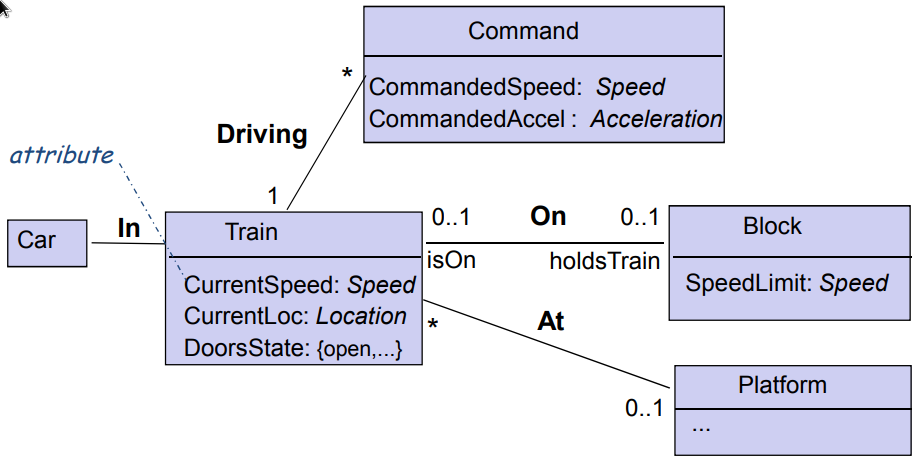
\includegraphics[width=0.7\textwidth]{images/association_diagram.png}
    \caption{\lr{Entities, Associations, Attributes in UML}}
\end{figure}

\begin{figure}[H]
    \centering
    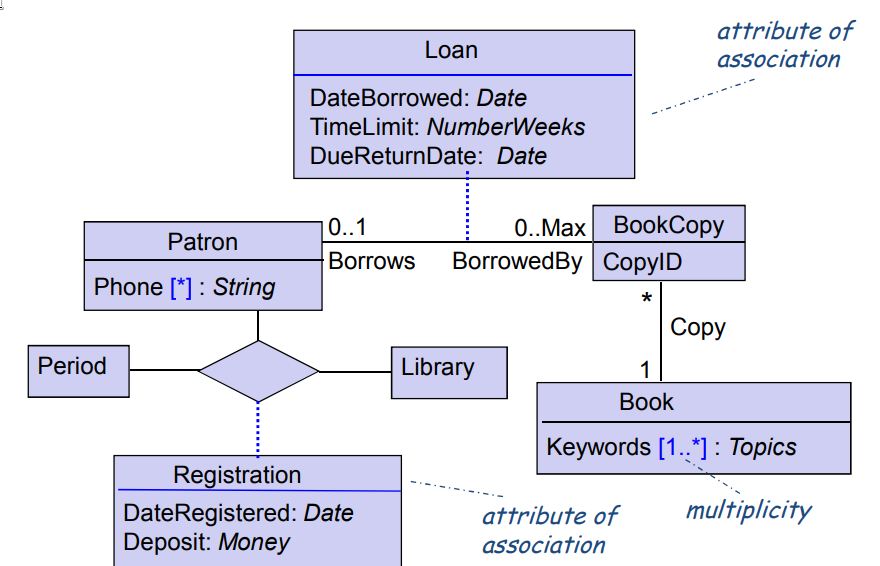
\includegraphics[width=0.7\textwidth]{images/association_diagram_2.png}
    \caption{\lr{Entities, Associations, Attributes more details in UML}}
\end{figure}

\subsubsection{\lr{Inheritance} یا وراثت}

در این نوع از روابط، رابطه بین کلاس‌ها به صورت والد و فرزندی می‌باشد که فرزندان
ممکن است برخی یا همه صفات کلاس والد را به ارث برده باشند یا برخی کلاس‌ها با توجه
به نیاز خود، صفات محدودتری را به ارث برده باشند. معمولاً این کلاس در قدم‌های
ابتدایی مسئله دیده می‌شود.

برای مثال، یک کتاب، یک محتوای آموزشی می‌باشد. همچنین یک فیلم نیز یک محتوای
آموزشی. در این مثال محتوای آموزشی را به عنوان کلاس والد در نظر می‌گیریم که
می‌تواند به شکل‌های مختلفی مانند فیلم یا کتاب نوشتاری ارائه شوند.

\subsubsection{\lr{Composition} یا ترکیب}

در این نوع رابطه، گاهی یک شئ مستقل نداریم، (برای مثال شئ‌ای به نام ماشین نداریم)
هویت یک کلاس با مهم‌ترین بخش‌های آن مشخص می‌شود. برای مثال یک پیام تشکیل شده از
۳ بخش مهم، بدنه، سرتیتر، فوتر. اگر این ۳ بخش به صورت یکپارچه در کنار هم باشند
ساختار اصلی پیام را تشکیل می‌دهند زیرا هر بخش به عنوان جز مستقل نمی‌باشد بلکه
رابطه کل به جز می‌باشد.

برای مثال \lr{Session} یک دستگاه \lr{ATM} رابطه کل به جز در خصوص واریزی‌ها و
تراکنش‌ها می‌باشد. زمانی که \lr{Session} یک کاربر (با خروج کارت) به پایان رسید،
\lr{Session} کاربر قبلی بایستی از بین برود \footnote{\lr{Distory}}. در حقیقت
باید ببینیم که نیاز سیستم چیست و چه زمانی اتفاق می‌افتد. این موارد به صورت
قانونی نیست بلکه به صورت تصمیم می‌باشد. در حقیقت در این بخش می‌تواند از افراد
خبره و متخصص این بخش استفاده کرد. حیات جز به حیات کل سیستم وابسته می‌باشد.

\subsubsection{\lr{Aggrigation} یا تجمیع}

این رابطه مشابه رابطه ترکیبی یا \lr{Composition} می‌باشد با این تفاوت که در
تجمیع بیان می‌شود که اگر کل از بین برود، اجزا باز هم باقی می‌ماند.

\begin{figure}[H]
    \centering
    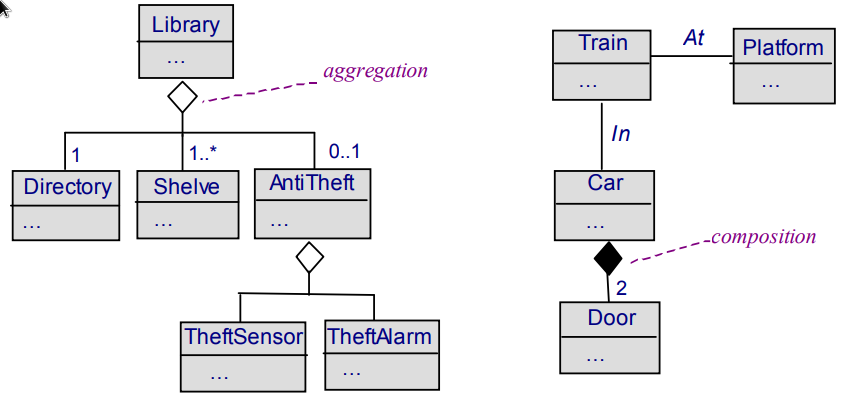
\includegraphics[width=0.7\textwidth]{images/aggregation_relation.png}
    \caption{\lr{Object aggregation: example}}
\end{figure}

\subsubsection{\lr{Multiplicity} یا تعدد}

در این رابطه، هر نمونه‌ای از یک کلاس با تعدادی از نمونه‌های کلاس دیگر ارتباط
دارند.

\begin{LTR}
    \begin{itemize}
        \item $[0..x]$: Optional attribute
        \item $[x..*]$: Attribute value = Set of values
        \item $[1..1]$: Mandatory attribute, single value: by default, omitted
        \item e.g. $phoneNumber$ $[0..*]$: String, optional possibly multiple
        values
    \end{itemize}
\end{LTR}

بر اساس دو اصل کار می‌کند، \lr{Prescriptive} و \lr{Descriptive}. در این رابطه
همه المان‌ها باید توجیه داشته باشند. اینکه فردی بتواند ۵ تا کتاب قرض بگیرد
می‌شود \lr{Prescriptive} و اینکه می‌خواهیم در هنگام قرض گرفتن شرط بگذاریم
\lr{System Requirement} می‌باشد. در حقیقت تعدد‌ها در سیستم توجیه‌پذیر هستند.

\subsection{کلاس انجمنی}

کلاس انجمنی یک کلاس مستقل می‌باشد و هیچ ربطی به رابطه انجمنی ندارد. با نقطه‌چین
به کلاس‌ها متصل می‌شود و بیشتر در کلاس‌های \lr{n} به \lr{n} مورد استفاده قرار
می‌گیرد. برای مثال، دانشجویی کتابی را قرض می‌گیرد و مهلت تحویل کتاب (\lr{Time
duration}) به مدت ۲ هفته می‌باشد. کلاس کتاب و کلاس دانشجو جدا می‌باشد و مقدار
\lr{Time duration} به عنوان صفت برای کتاب یا دانشجو تعریف نمی‌شود بلکه به عنوان
یک کلاس انجمنی بیان می‌شود. یعنی صفتی از کلاس انجمنی خواهد بود.

در مثالی دیگر یک سیستم فایل اشتراکی داریم که دانشجویان مختلفی می‌توانند به آن
دسترسی داشته باشند. سطح دسترسی را به عنوان صفت دانشجو در نظر نخواهیم گرفت بلکه
به نیاز به تعریف یک کلاس انجمنی داریم تا بتوانیم مشخص کنیم که چه کاربری
(دانشجویی) به چه فایلی (کلاس دیگر) چه دسترسی دارد.

\begin{LTR}
    \lr{Ali(sid, Ali, other properties);}

    \lr{Book1(bid, Book1, other properties);}

    \lr{Association(id, sid, bid, (access: type of "R|W"));}
\end{LTR}

\subsection{نکات پایانی}

\begin{itemize}
    \item هر نمادی بایستی به هدف متصل شود.
    \item از تعریف هدف تمام این المان‌ها را بدست می‌آوریم.
    \item همه المان‌ها به کلاس ارتباط دارند.
    \item گاهی فعل "شامل شدن" می‌باشد و \lr{on} یا \lr{Follow} کردن نیست بلکه
    باید به صورت ترکیبی یا تجمیعی دیده شوند.
    \item همه \lr{Domain property}ها تعدد را بیان نمی‌کنند.
    \item می‌تواند چیز اضافی در سبد وجود داشته باشد چرا که ممکن است یک سیستم
    جامع از پیش طراحی شده را در سیستم جاری بخواهیم الگو برداری کنیم که به یکسری
    چیزاش نیاز داریم به یسری چیزاش نیاز نداریم و آن را کنار می‌گذاریم.
\end{itemize}
% \newpage

\section{فصل یازدهم}

\section(\lr{Agent Diagram})

از این بخش سوال امتحانی خواهیم داشت.

عامل‌ها براساس وظایفشون مشخص میشه چی رو ببین و چی رو نبینن.

با تحمیل زنجیره آسیب مشخص میشه که تو ایجنت فعلی که داریم استفاده میکنم یا غلط
دادیم وظیفه رو یا تو انجام وظیفش تخوب نیست باید به عامل دیگه‌ای بدیمش.

کنترل یک ایجنت مانیتور یه ایجنت دیگست.

سه دسته دیاگرام عامل داریم:

Agent diagram کامل ترینه که گول داریم اجینت داریم و کلاس داریم.

Context diagram: همون مجموعه ارتباطی آسامپشن‌ها و غیره هستند.

depedency diagram: برای زنجیره آسیبه

اسلاید هشت فایل ۱۱

Ag1

مسئول یه گوله

زنجیره آسیب ارتباطات اینتپونت هر عامل دیگر را مشخص میکند.

همیشه از انتها به ابتدا می‌خوانیم.

تمرین:

در یک مثال یک گول در نظر بگیرید و یک زنجیره آسیب براش بسازید.

نوشته می‌شود. (نسبت به سکشن‌هایی بالایی ببین ببخشید واقعاً)

نهاد کلاس‌های تغییر میکند.

بقیش دیگه تو طراحی می‌مونه

قط کلاس‌ها و اتریبیوت‌های که از قضای مسئله می‌آیند.

\newpage
\listoffigures
\listoftables
\end{document}